\documentclass{article}
\usepackage[utf8x]{inputenc}
\usepackage{agda}
\usepackage[nocenter]{qtree}
\usepackage{amssymb,amsthm,amsmath}
\usepackage{fullpage}
\usepackage{url}
\usepackage{comment}
\usepackage{tikz}
\usepackage{tikz-cd}
\usepackage{listings}
\usepackage{multicol}
\usepackage{amsmath}
\usepackage{stmaryrd}
\usepackage{proof}
\usetikzlibrary{quotes,fit,positioning}
\tikzset{>=latex}

%%%%%%%%%%%%%%%%%%%%%%%%%%%%%%%%%%%%%%%%%%%%%%%%%%%%%%%%%%%%%%%%%
%% Macros

\newtheorem{theorem}{Theorem}[section]
\newtheorem{lemma}[theorem]{Lemma}
\newtheorem{definition}[theorem]{Definition}
\newtheorem{proposition}[theorem]{Proposition}
\newtheorem{corollary}[theorem]{Corollary}

\newcommand{\inkscape}[2][1.5]{
\begin{center}
\scalebox{#1}{
\includegraphics{inkscape/#2}
}
\end{center}
}

\newcommand{\nboxtimes}[2]{\,\,~{^{#1}\boxtimes^{#2}}~\,\,}
\newcommand{\mm}{\texttt{\textminus}}
\newcommand{\pp}{\texttt{+}}
\newcommand{\inl}[1]{\textsf{inl}~#1}
\newcommand{\inr}[1]{\textsf{inr}~#1}
\newcommand{\cp}[3]{#1\stackrel{#2}{\bullet}#3}
\newcommand{\idt}[3]{#2 \equiv_{#1} #3}
\newcommand{\idrt}[3]{#3 \equiv_{#1} #2}
\newcommand{\refl}[1]{\textsf{refl}~#1}
%% \newcommand{\lid}{\textsf{lid}}
\newcommand{\alt}{~|~}
%% \newcommand{\rid}{\textsf{rid}}
\newcommand{\linv}{l!}
\newcommand{\rinv}{r!}
\newcommand{\invinv}{!!}
\newcommand{\assoc}{\circ}
\newcommand{\identlp}{\ensuremath{\mathit{unite}_+\mathit{l}}}
\newcommand{\identrp}{\ensuremath{\mathit{uniti}_+\mathit{l}}}
\newcommand{\identlsp}{\ensuremath{\mathit{unite}_+\mathit{r}}}
\newcommand{\identrsp}{\ensuremath{\mathit{uniti}_+\mathit{r}}}
\newcommand{\swapp}{\ensuremath{\mathit{swap}_+}}
\newcommand{\assoclp}{\ensuremath{\mathit{assocl}_+}}
\newcommand{\assocrp}{\ensuremath{\mathit{assocr}_+}}
\newcommand{\identlt}{\ensuremath{\mathit{unite}_*\mathit{l}}}
\newcommand{\identrt}{\ensuremath{\mathit{uniti}_*\mathit{l}}}
\newcommand{\identlst}{\ensuremath{\mathit{unite}_*\mathit{r}}}
\newcommand{\identrst}{\ensuremath{\mathit{uniti}_*\mathit{r}}}
\newcommand{\swapt}{\ensuremath{\mathit{swap}_*}}
\newcommand{\assoclt}{\ensuremath{\mathit{assocl}_*}}
\newcommand{\assocrt}{\ensuremath{\mathit{assocr}_*}}
\newcommand{\absorbr}{\ensuremath{\mathit{absorbr}}}
\newcommand{\absorbl}{\ensuremath{\mathit{absorbl}}}
\newcommand{\factorzr}{\ensuremath{\mathit{factorzr}}}
\newcommand{\factorzl}{\ensuremath{\mathit{factorzl}}}
\newcommand{\dist}{\ensuremath{\mathit{dist}}}
\newcommand{\factor}{\ensuremath{\mathit{factor}}}
\newcommand{\distl}{\ensuremath{\mathit{distl}}}
\newcommand{\factorl}{\ensuremath{\mathit{factorl}}}
%% \newcommand{\distz}{\mathit{absorbr}}
\newcommand{\iso}{\leftrightarrow}
\newcommand{\proves}{\vdash}
\newcommand{\idc}{\mathit{id}\!\!\leftrightarrow}
\newcommand{\Rule}[4]{
\makebox{{\rm #1}
$\displaystyle
\frac{\begin{array}{l}#2 \\\end{array}}
{\begin{array}{l}#3      \\\end{array}}$
 #4}}
\newcommand{\jdg}[3]{#2 \proves_{#1} #3}
\newcommand{\sem}[1]{\ensuremath{\llbracket{#1}\rrbracket}}

% Unicode declarations

\DeclareUnicodeCharacter{9678}{\ensuremath{\odot}}
\DeclareUnicodeCharacter{9636}{\ensuremath{\Box}}
%% shorten the longarrow
\DeclareUnicodeCharacter{10231}{\ensuremath{\leftrightarrow}}

% TIKZ declarations
\tikzstyle{func}=[rectangle,draw,fill=black!20,minimum size=1.9em,
  text width=2.4em, text centered]

% Parts of the document itself

\title{Embracing the Laws of Physics: \\ Three Reversible Models of Computation}
\author{Jacques Carette \qquad\qquad Roshan P. James \qquad\qquad Amr Sabry \\
McMaster University \qquad\qquad Google \qquad\qquad Indiana University}

\newtheorem{thm}{Theorem}[section]
\newtheorem{defn}{Definition}[section]
\newtheorem{prop}{Proposition}[section]

\newcommand{\amr}[1]{\fbox{Amr says:} \textbf{#1}}
\newcommand{\jc}[1]{\fbox{Jacques says:} \textbf{#1}}
\newcommand{\roshan}[1]{\fbox{Roshan says:} \textbf{#1}}

\newcommand{\lcal}{\ensuremath{\lambda}-calculus}

\newcommand{\fin}[1]{\ensuremath{\left[#1\right]}}
\newcommand{\Nat}{\ensuremath{\mathbb{N}}}
\newcommand{\true}{\mathit{true}}
\newcommand{\false}{\mathit{false}}
\newcommand{\Gpd}{\ensuremath{\mathsf{Groupoid}}}

\newcommand{\kw}[1]{{\scriptsize{\textbf{\texttt{#1}}}}}
\newcommand{\ctr}[1]{{\scriptsize{\texttt{#1}}}}
\newcommand{\inline}[3]{\ctr{#1} \textasciitilde \ctr{#2}:\ctr{#3}}

\begin{document}
\maketitle

\begin{abstract}
  Our main models of computation (the Turing Machine and the RAM) and
  most modern computer architectures make fundamental assumptions
  about which primitive operations are realizable on a physical
  computing device. The consensus is that these primitive operations
  include logical operations like conjunction, disjunction and
  negation, as well as reading and writing to a large collection to
  memory locations. This perspective conforms to a macro-level view of
  physics and indeed these operations are realizable using macro-level
  devices involving thousands of electrons. This point of view is
  however incompatible with computation realized using quantum devices
  or analyzed using elementary thermodynamics as both these
  fundamental physical theories imply that information is a conserved
  quantity of physical processes and hence of primitive computational
  operations.

  Our aim is re-develop foundational computational models in a way
  that embraces the principle of conservation of information. We first
  define what information is and what its conservation means in a
  computational setting. We emphasize the idea that computations must
  be reversible transformations on data. One can think of data as
  modeled using topological spaces and programs as modeled by
  reversible deformations of these spaces. We then illustrate this
  idea using three notions of data and their associated reversible
  computational models. The first instance only assumes unstructured
  finite data, i.e., discrete topological spaces. The corresponding
  notion of reversible computation is that of permutations. We show
  how this simple model subsumes conventional computations on finite
  sets. We then consider a modern structured notion of data based on
  the Curry-Howard correspondence between logic and type theory. We
  develop the corresponding notion of reversible deformations using a
  sound and complete programming language for witnessing type
  isomorphisms and proof terms for commutative semirings.  We then
  ``move up a level'' to examine spaces that treat programs as data
  which is a crucial notion for any universal model of computation. To
  derive the corresponding notion of reversible programs between
  programs, i.e., reversible program equivalences, we look at the
  ``higher dimensional'' analog to commutative semirings: symmetric
  rig groupoids. The coherence laws for these groupoids turn out to be
  exactly the sound and complete reversible program equivalences we
  seek.

  We conclude with some possible generalizations inspired by homotopy
  type theory and survey several open directions for further research.

%%  Something about Theseus?
\end{abstract}

% * Reversibility intro / motivation as we  have now more or less

% * Thesis statement: programs are reversible deformations on data /
%    spaces, almost necessarily by definition

% * Focus now is on data

% * If data is plain finite sets, programs become permutations (deformations on finite sets).

% * If data is structured trees, we get Pi.

% * Explain Pi with examples.

% * If data is itself deformations-on-finite-sets, then the
%   deformations between them become something quite
%   interesting. Explain Pi level 2 with examples.

% * Conclude with thoughts regarding other kinds of data that can be
%   plugged in into that story.

%%%%%%%%%%%%%%%%%%%%%%%%%%%%%%%%%%%%%%%%%%%%%%%%%%%%%%%%%%%%%%%%%
\section{Reversibility, the Missing Principle}

What kind of operations can computers perform? This question was
answered several times in the last hundred years, where each answer
proposes an abstract \emph{model of computation} that specifies
allowable operations and (usually) their cost. The emerging consensus,
reflected in both early models of computations such as the Turing
Machine and the RAM as well as in the early Von Neumann models and in
modern computer architectures, is that basic computer operations
include logical operations like conjunction, disjunction, and
negation, as well as reading from and writing to a large (infinite)
collection of memory locations. From this small set of primitive
operations emerges all higher-level programming languages and
abstractions.

No doubt, this consensus on the available primitive physical
operations has been successful. And no doubt, these operations
\emph{can} indeed be performed on a computer. Yet, today, with a
possible quantum computing revolution in sight and with unprecedented
explosion in embedded computers and cyber-physical systems, there are
reasons to re-think this foundational question again. In fact, the
calls to re-think this foundational question have been proclaimed by
physicists more than forty years ago as the following two quotes
testify:

\begin{quote}
  \textbf{Toffoli 1980~\cite{toffoli:1980}:} Mathematical models of
  computation are abstract constructions, by their nature unfettered
  by physical laws. However, if these models are to give indications
  that are relevant to concrete computing, they must somehow capture,
  albeit in a selective and stylized way, certain general physical
  restrictions to which all concrete computing processes are
  subjected.

  \textbf{Feynman 1982~\cite{springerlink:10.1007/bf02650179}:}
  Another thing that has been suggested early was that natural laws
  are reversible, but that computer rules are not. But this turned out
  to be false; the computer rules can be reversible, and it has been a
  very, very useful thing to notice and to discover that. This is a
  place where the relationship of physics and computation has turned
  itself the other way and told us something about the possibilities
  of computation. So this is an interesting subject because it tells
  us something about computer rules.
\end{quote}

\noindent These quotes by Toffoli and Feynman both highlight the
consequences of two obvious observations: (i) all the operations that
a computer performs reduce to basic physical operations; and (ii)
there is a mismatch between the logical operations of a typical model
of computation (which are logically irreversible) and the fundamental
laws of physics (which are reversible). One could certainly dismiss
the mismatch as irrelevant to the practice of computing but our thesis
is that the next computing revolution is likely to be founded on
revised models of computation that are designed to be in closer harmony
with the laws of physics.

After a detailed introduction on the origins of ``logically
reversibile computer operations'' and an excursion into the origins of
``irreversible computer operations,'' we will develop in detail three
reversible models of computation and discuss their potential
applications.

%%%%%%%%%
\paragraph*{Maxwell's Daemon.}
To fully appreciate the missing principle of ``reversibility'' in
conventional computing, we go back to an old thought experiment by
J. C. Maxwell. The details are codified in a letter that Maxwell wrote
to P. G Tait in 1867 -- the letter, whose ideas are now known as
\emph{Maxwell's Daemon}, tells of a thought experiment that seems to
indicate that intelligent beings can somehow violate the second law of
thermodynamics, thereby violating physics itself. Many resolutions
were offered for this conundrum (for a compilation, see the book by
Leff and Rex~\cite{leff1990}), but none withstood careful scrutiny
until the establishment of \emph{Landauer's Principle} in
1961~\cite{Landauer:1961} -- a principle whose experimental validation
happened recently in 2012~\cite{berut2012experimental}.

Maxwell's daemon appears to violate the second law of thermodynamics by
having a tiny ``intelligence'' observing the movement of individual
particles of a gas and separating fast moving particles from slow
moving ones, thereby reducing the total entropy of the
system. Landauer's resolution of the daemon relied on two ideas that
took root only a few decades earlier: the formal notion of computation
(through the work of Turing~\cite{turing}, Church~\cite{church51}, and
others) and the formal notion of information (through the work of
Shannon~\cite{shannon1948}). Landauer reasoned that the computation
done by the finite brain of the daemon, involves getting information
about the movement of molecules, storing that information, analyzing
that information to act on it, and then --- and this is the critical
step --- overwriting it to make room for the next computation.  In
other words, the computation that is manipulating information in the
daemon's brain \textit{must be thermodynamic work}, thereby bringing
the daemon back into the fold of physics.

This is a strange and wonderful idea: information, physics, and
computation are inextricably linked. In contrast, when the early
models of computation were developed, there was no compelling reason
to take the information content of computations into consideration
-- in fact, at that time there was no quantifiable notion of
information. These models followed in the footsteps of logic where,
following hundreds of years of tradition, the truth of a statement was
seen as ``absolute'' and independent of any reasoning, understanding,
or action. Statements were either true or false with no regard to any
``observer'' and the idea that statements had information content that
should be preserved was outside the classical understanding of
logic. Hence the fact that conventional logic operations such as
conjunction and disjunction were logically irreversible and hence lose
information was not a concern. Landauer's observation implied however
that ideas in each field have consequences for the
other~\cite{bennett:1973:lrc,bennett1985fundamental,bennett2010notes,bennett2003notes,baker:1992:nft,baez2011physics,dblp:conf/csfw/malacarias12}. To
really appreciate this fact, we delve deeper into the origin of our
computational models and argue that they are essentially reflections
of contemporary laws of physics.

%%%%%%%%%
\paragraph*{Origins of Computational Models.}
Current high-level programming languages as well as current hardware
are both based on the mathematical formalization of logic developed by
De Morgan, Venn, Boole, and Peirce in the mid to late 1800s. Going
back to Boole's 1853 book entitled \emph{An Investigation of the Laws
  of Thought, on which are Founded the Mathematical Theories of Logic
  and Probabilities}, we find that the opening sentence of Ch.~1 is:
\begin{quote}
  The design of the following treatise is to investigate the fundamental laws
  of those operations of the mind by which reasoning is performed;
\end{quote}
which clearly identifies the ``source'' of the logical laws as
mirroring Boole's understanding of human reasoning. A few chapters
later, we find:
\begin{quote}
  \textbf{Proposition IV.}  That axiom of metaphysicians which is termed the
  principle of contradiction, and which affirms that it is impossible for any
  being to possess a quality, and at the same time not to possess it, is a
  consequence of the fundamental law of thought, whose expression is $x^2 =
  x$.
\end{quote}
This ``law'' is reasonable in a classical world but is violated by the
postulates of quantum mechanics. Although a detailed historical
analysis of Boole's ideas in the light of modern physics is beyond our
scope, the above quotes should convey the idea that our elementary
computing notions date back to ideas that were thought reasonable in
the late 1800s.

Machines that ``compute'' are quite old. M\"{u}ller (1786) first
conceived of the idea of a ``difference machine,'' which Babbage
(1819--1822) was able to construct. There are other computer
precursors as well -- the first stored programs were actually for
looms, most notably those of Bouchon (1725) which operated on a paper
tape, and Jacquard (1804) which operated by chains of punched cards.
But it was only in the 20th century that computer science emerged as a
formal discipline. One of the pioneering works was Alan Turing's
seminal paper~\cite{turing} in 1936 which established the idea that
computation has a formal interpretation and that all computability can
be captured within a formal system. Implicit in this achievement
however is the idea that abstract models of computation are just that
-- \emph{abstractions of computation realized in the physical world.}
Indeed, going back to Turing's 1936 article \emph{On Computable
  Numbers, with an Application to the Entscheidungsproblem,}, the
opening sentence of Sec. 1 is:
\begin{quote}
  We have said that the computable numbers are those whose decimals
  are calculable by finite means [\ldots] the justification lies in
  the fact that the human memory is necessarily limited.
\end{quote}
In Sec. 9, we find:
\begin{quote}
  I think it is reasonable to suppose that they can only be squares
  whose distance from the closest of the immediately previously
  observed squares does not exceed a certain fixed amount.
\end{quote}
It is worth noting that these assumptions are both physical (on
distances) and metaphysical (on restrictions of the mind).  If we take
the human mind to be a physical ``machine'' which does computation,
then when both of the above assumptions are translated to the language
of physics, they embody what is known as the ``Bekenstein
bound''~\cite{PhysRevD.23.287}, which is an upper limit on the amount
of information that can be contained within a given finite region of
space. A detailed historical account of these ideas in the context of
modern physics is again beyond our scope. However, the quotes above,
like the ones before, should convey the ideas that our theories of
computation and complexity are based on some physical assumptions that
Turing and others found reasonable in the 1930s.

To summarize, a major achievement of computer science has been the
development of abstract models of computation that shield the
discipline from rapid changes in the underlying technology. Yet, as
effective as these models have been, one must note that they
\emph{embody several implicit physical assumptions} and these
assumptions are based on a certain understanding of the laws of
physics. Our understanding of physics has evolved tremendously since
1900!  Thus it is time to revisit these abstractions, especially with
respect to quantum mechanics.  Indeed one should take the physical
principles underlying quantum mechanics, the most successful physical
theory known to us and adapt computation to ``learn'' from these
principles.  In the words of Girard~\cite{Girard:2007:TMI:1348911.1348915}:
\begin{quote}
  In other terms, what is so good in logic that quantum physics should
  obey?  Can't we imagine that our conceptions about logic are wrong,
  so wrong that they are unable to cope with the quantum miracle?
  [\ldots] Instead of teaching logic to nature, it is more reasonable
  to learn from her. Instead of interpreting quantum into logic, we
  shall interpret logic into quantum.
\end{quote}

There are, in fact, many different quantum mechanical principles which
are at odds with our current models of computation. In this paper, we
will focus on the previously identified principle of
\emph{reversibility}. In more detail, we will view data as an explicit
representation of \emph{information} and programs as processes that
transform information in a reversible way, i.e., processes that are
subject to the physical principle of \emph{conservation of
  information.} We will formalize this idea and follow its
consequences, which will turn out to be far reaching.

%%%%%%%%%
\paragraph*{Programs as Reversible Deformations.}
To better understand the essence of ``conservation of information'' in
the context of computing, we first look for analogous ideas in
physics, but this time at the macro scale. Viewing information as a
physical object, what does it mean to transform an object in such a
way that we do not lose its fundamental character?

For rigid objects (like a chair), the only such transformations are
translations and rotations. But what about something more flexible,
with multiple representations, such as a water balloon?  Such objects
can be \emph{deformed} in various ways, but still retain their
fundamental character -- as long as we do not puncture them or
over-stretch them. Ignoring material characteristics
(i.e. over-stretching), what is special about these deformations, as
well as for translations and rotations, is that they correspond to
continuous maps, with a continuous inverse. In fact, even more is
true: they are analytic maps, with analytic inverses. For our purpose,
the most important part is that such maps are infinitely
differentiable.  In other words, not only is there an inverse to the
deformation, but its derivative is also invertible, and so on.

When we look around, we find many different words for related
concepts: isomorphism, equivalence, sameness, equality,
interchangeability, comparability, and correspondence, to name a
few. Some of these are informal concepts, while others have formal
mathematical meaning.  More importantly, even amongst the formal
concepts, there are differences -- which is why there are so many of
them! Because there are many such notions, we also need to walk our
way through them to find the one which is ``just right.'' Thus we seek
a concept which is neither too strong nor too weak, that will express
when some structured information should be treated as ``the same.''
We can draw an analogy with topology: in topology, all point sets can
always be equipped with either the discrete or the indiscrete
topology, but both of these extremes are rarely useful. We will
develop our working notion of ``sameness'' as we go through the
various components that make up a programming language.

Starting from the physical perspective, whatever our notion of data
is, we will be interested in programs as representing transformations
of that data which are reversible. In other words, we want our
programs-as-transformations to ``play well'' with the inherent notion
of ``sameness'' that our data will carry. Thus we need to start by
looking at what structure our data has, and that will help us define
an appropriate notion of a reversible program. Of course, when
programs themselves are data, things do get more complicated.  In the
following sections, we will look at different natural classes of data,
and explore the corresponding notion of reversible programs.

To summarize, we will take ``the same'' as a fundamental principle and
derive what it means for data, programs, program transformations, as
well as proofs / deductions, to be ``the same'' -- in an manner
consistent with preservation of information. This stands in stark
contrast with most current approaches to reversible computation, which
start from current models of computation involving irreversible
operations and try to find various ways to \emph{patch things up} so
as to be reversible.

\amr{We should also have a quick survey of other works in reversible
computation? Most of the other work tries to start from well known
models of computation or well known programming languages, and then
adapts them to be reversible. Pi is different in that it starts from
the semantic implications of reversibility. Then, because it adds
types, rather than control-flow (or even data-flow) as its next layer
of ``understanding,'' this leads to equivalences, isomorphisms, etc.
This then leads, quite naturally, to finding that the ``proof
language'' of semirings (and Rig Groupoids at level 2) is actually a
programming language. And it is Pi. This is a neat twist on
Curry-Howard because CH is about \textbf{inhabitation} only. But with
``conservation of information'' as the basis, a different kind of
correspondence arises; in fact, this one may well be an actual
isomorphism.}

\jc{I think it would be fair to have a \textit{quick} survey
of other works. The most important aspect would be to draw out that
they all start from known models of computation and then attempt to
make them reversible.  Our originality is to start from the semantics
of reversibility (even further back, preservation of information)
and derive a programming language purposefully designed to denote
exactly that. Having said that, I am not in a good position to
write such a survey, being the least knowledgeable of all 3 of us
of this general area.}

%%%%%%%%%%%%%%%%%%%%%%%%%%%%%%%%%%%%%%%%%%%%%%%%%%%%%%%%%%%%%%%%%
\section{Data I: Finite Sets}
\label{sec:dataone}

Most programming languages provide primitive data like booleans,
characters, strings, and (bounded) numbers that are naturally modeled
as finite sets. We therefore start by modeling reversible computations
over finite and discrete spaces of points. Infinite sets are more
subtle, and will be discussed in the conclusion.

What does it mean to deform a space of points? For example, what
transformation can we do on a bag of marbles? Well, we can shuffle
them around and that is the only transformation that will preserve the
space. Turning to the mathematical abstraction as sets, we ask what
does it mean for two finite sets to be ``the same''?  Well, clearly
the sets $A = \left\{1, 2, 3\right\}$ and $B = \left\{c, d\right\}$
are different.  Why?  Well, suppose there was a transformation
$f : A \rightarrow B$ that deformed $A$ into $B$, and another
$g : B \rightarrow A$ which undid this transformation. Since $f$ is
total, by the pigeonhole principle, two elements of $A$ would be
mapped to the same element of $B$. Suppose that this is $2$ and $3$,
and that they both map to $d$.  But $g(d)$ cannot be both $2$ and $3$,
and so $g$ is not the inverse of $f$. With just a little more work, we
can show that $f$ (and $g$) must be both injective and surjective. In
other words, $f$ (and $g$) must be a bijection between $A$ and $B$.
And of course this only happens when $A$ and $B$ have the same number
of elements. More importantly, given a bijection $f : C \rightarrow D$
of finite sets $C,D$, there always exists another bijection
$g : D \rightarrow C$ which is $f$'s inverse. So, for finite sets,
\emph{bijections} act as reversible deformations.

This discussion is purely ``semantic,'' in the sense that it is about
the denotation of simple primitive data (sets) and their reversible
deformations (bijections).  We would like to reverse engineer a programming
language from this denotation. But first, an obvious remark: any two sets
$C$ and $D$ of cardinality $n$ are always in bijective correspondence. So
we can abstract away from the details of the elements of $C$ and $D$ and
instead choose canonical representations -- in much the same way as computers
choose binary words to represent everything.

\begin{defn} For $n\in\Nat$, denote by $\fin{n}$ the set
$\left\{0,1,\ldots,n-1\right\}$.
We will refer to $\fin{n}$ as the canonical set with $n$ elements.
\end{defn}

Bijections on \fin{n} have a specific name: permutations. As is
well-known, permutations can be generated by sequential compositions of
transpositions. Thus we can create a small language for writing
permutations on $\fin{n}$ as
\[\begin{array}{rcl}
p^n &::=& \mathit{id} ~\mid~ \mathit{swap}~i~j ~\mid~ p^n \fatsemi p^n
  \end{array}\]
where $i,j:\Nat$, $i\neq j$ and $i,j < n$. Note that we could remove
$\mathit{id}$ from the language and drop the $i\neq j$ condition so that
$\mathit{swap}~j~j$ would represent the identity permutation.

For convenience, we write $[2^n]$ for the finite set representing
$n$-bit words with the canonical ordering for binary numbers. Thus
when $n=3$, the finite set has elements $\{0,1,2,3,4,5,6,7\}$ which
correspond to the 3-bit words $\{000,001,010,011,100,101,110,111\}$.
Although this language appears weak, it is universal for reversible
boolean combinational circuits $[2^i] \rightarrow [2^i]$ with $i$
input/output wires.

To illustrate the expressiveness of the language, we develop a few
small examples. We start by writing boolean negation ``not'' as a
permutation $[2^1] \rightarrow [2^1]$, the controlled-not gate (also
known as ``cnot'') as a permutation $[2^2] \rightarrow [2^2]$, and the
controlled-controlled-not gate (also known as ``toffoli'') as a
permutation $[2^3] \rightarrow [2^3]$:
\[\begin{array}{rcl}
\mbox{not} &=& \mathit{swap}~0~1 \\
\mbox{cnot} &=& \mathit{swap}~2~3 \\
\mbox{toffoli} &=& \mathit{swap}~6~7
\end{array}\]
The ``cnot'' gate operates on two bits and negates the second (the
target bit) if the first one (the control bit) is 1, i.e., it swaps
$10$ and $11$; the ``toffoli'' gate negates the third bit (the target
bit) if both the first two bits (the control bits) are 1, i.e., it
swaps $110$ and $111$.

There is however a subtle issue: programming in such an unstructured
language is \emph{not} compositional in the sense that using the
``not'' gate in a larger circuit forces us to change its
implementation. Indeed if we had two bits and wanted to use ``not'' to
negate the first bit, we would write the permutation of type
$[2^2] \rightarrow [2^2]$ that permutes $00$ with $10$ \emph{and}
permutes $01$ with $11$, i.e, the permutation
$\mathit{swap}~0~2 \fatsemi \mathit{swap}~1~3$. To illustrate
how inconvenient this is, consider the reversible full adder
below designed by Desoete et al.~\cite{117414}:

\begin{center}
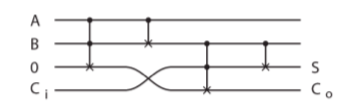
\includegraphics[scale=0.6]{full-adder.png}
\end{center}

In the figure (copied from a more general paper that includes
alternative designs~\cite{Rentergem2005OptimalDO}), the full adder
takes 4 inputs: the two bits to add $A$ and $B$, an incoming carry bit
$C_i$, and a heap input initialized to 0 to maintain
reversibility. There are four outputs: the first two are identical to
the incoming bits $A$ and $B$ and are considered ``garbage.'' The
third bit $S$ is the sum and the last bit $C_o$ is the outgoing carry
bit. In the notation used to describe the circuit, the $\times$ denotes
boolean negation, the dots are control bits. In our reversible
language, we can express this circuit as the following permutation of
type $[2^4] \rightarrow [2^4]$:

\begin{equation}\label{eq:adder}
\begin{array}{l@{\hspace{1cm}}l}
\mathit{swap}~12~14 \fatsemi \mathit{swap}~13~15 ~\fatsemi & \mbox{toffoli} \\
\mathit{swap}~8~12 \fatsemi \mathit{swap}~9~14 \fatsemi
    \mathit{swap}~10~13 \fatsemi \mathit{swap}~11~15 ~\fatsemi & \mbox{cnot and swap} \\
\mathit{swap}~6~7 \fatsemi \mathit{swap}~14~15 ~\fatsemi & \mbox{toffoli} \\
\mathit{swap}~4~6 \fatsemi \mathit{swap}~5~7 \fatsemi
    \mathit{swap}~12~14 \fatsemi \mathit{swap}~13~15 & \mbox{cnot}
\end{array}
\end{equation}

Note how the implementation of $\mathit{cnot}$ as a permutation
$[2^2] \rightarrow [2^2]$ cannot be directly reused in the larger
circuit $[2^4] \rightarrow [2^4]$.

For such reasons, in programming practice we are interested in
structured data and compositional abstractions, which will be the
subject of the next section. What we do learn from this short investigation
using untyped and unstructured sets is what the ``\emph{purely
  operational}'' view of the theory would be. In particular, it tells
us that permutations are an inescapable part of the fabric of
reversible computing.  However as permutations are untyped, and act on
the canonicalized version of $n$-element sets (i.e. those sets where
all the structure has been forgotten), these are a rather pale shadow
of the rich tapestry of information-preserving transformations of
structured data, which we investigate next.

%%%%%%%%%%%%%%%%%%%%%%%%%%%%%%%%%%%%%%%%%%%%%%%%%%%%%%%%%%%%%%%%%
\section{Data II: Structured Finite Types}
\label{sec:pi1}

Instead of spaces (aka discrete sets) consisting solely of
unstructured isolated points, we now investigate structured spaces
built from sums and products of elementary spaces. This structure
corresponds to the building blocks of type theory which are: the empty
type ($\bot$), the unit type ($\top$), the sum type ($\uplus$), and
the product ($\times$) type. Before getting into the formal theory,
let's consider possible deformations on the space $(\top \uplus \bot)
\times (\top \uplus \top)$. This space is the product of two
subspaces: the subspace $(\top \uplus \bot)$ which itself is the sum
of the space~$\top$ containing one element $\texttt{tt}$ and the empty
space $\bot$ and the subspace $(\top \uplus \top)$ which is the sum of
two spaces each containing the one element $\texttt{tt}$. First, as
discussed in the previous section, any deformation of this space must
at least preserve the number of elements: we can neither create nor
destroy points during any continuous deformation. Seeing that the
number of elements in our example space is 2, a reasonable hypothesis
is that we can deform the space above to any other space with 2
elements such as $\top \uplus \top$ or $\top \uplus (\top \uplus
\bot)$. What this really means is that we are treating the sum and
product structure as malleable. For example, imagining a product
structure as arranged in a grid; by ``stretching'' we can turn it
in to a sum structure arranged in a line. We can also change the
orientation of the grid by exchanging the axes, as well as do other
transformations --- as long as we preserve the number of points.
Of course, it is not a priori clear that this necessary requirement
is also sufficient.  Making this intuition precise will be the topic of this
section.

%%%%%%%%%
\subsection{A Model of Type Equivalences}

We now want a proper mathematical description of this idea. Our goal
is a denotational semantics on types which makes types that have the
same number of points be equivalent types.  First we note that the
structure of types has a nice correspondence (Curry-Howard) to logic:

\begin{center}
\begin{tabular}{c|c}
Logic & Types \\ \hline
$\false$ & $\bot$ \\
$\true$ & $\top$ \\
$\land$ & $\times$ \\
$\lor$ & $\uplus$ \\
\end{tabular}
\end{center}

\noindent This correspondence is rather fruitful. As logical
expressions form a commutative semiring, we would expect that types
too form a commutative semiring. And indeed they do -- at least up to
\emph{type isomorphism}.  The natural numbers $\Nat$ are another
commutative semiring; it will turn out that, even though the
Curry-Howard correspondence has been extremely fruitful for
programming language research, it is $\Nat$ which will be a better
model for finite structured types as the corresponding commutative
semiring captures the familiar numerical identities that preserve the
number of points in the types.

\begin{defn}
\label{def:rig}
A \emph{commutative semiring} (sometimes called a \emph{commutative
  rig} --- commutative ri\emph{n}g without negative elements)
$(R,0,1,+,\cdot)$ consists of a set $R$, two distinguished elements of
$R$ named $0$ and $1$, and two binary operations~$+$ and $\cdot$,
satisfying the following relations for any $a,b,c \in R$:
\[\begin{array}{rcl}
0 + a &=& a \\
a + b &=& b + a \\
a + (b + c) &=& (a + b) + c \\
\\
1 \cdot a &=& a \\
a \cdot b &=& b \cdot a \\
a \cdot (b \cdot c) &=& (a \cdot b) \cdot c \\
\\
0 \cdot a &=& 0 \\
(a + b) \cdot c &=& (a \cdot c) + (b \cdot c)
\end{array}\]
\end{defn}

\begin{prop}
The structure $\left(\Nat, \false, \true, \lor, \land\right)$
is a commutative semiring.
\end{prop}

We would like to adapt the commutative semiring definition to the
setting of structured types. First, types do not naturally want to be
put together into a ``set.''  This can be fixed if we replace the set
$R$ with a universe $U$, and replace the set membership $0 \in R$ with
the typing judgement $\bot : U$ (and similarly for the other
items). Our next instinct would be to similarly replace $=$ with a
type $A \equiv B$ that asserts that $A$ and $B$ are \emph{propositionally
equal}, i.e. reduce to equivalent type-denoting expressions under the rules of
the host type system.  This is however not true: the
proposition $A \times B \equiv B \times A$ is not
normally\footnote{Except in univalent type theory where equivalent
types are identified.} provable for arbitrary types $A$ and $B$. But
it should be clear that $A \times B$ and $B \times A$ contain
equivalent information. In other words, we would like to be able to
witness that $A \times B$ can be reversibly deformed into $B \times
A$, and vice-versa. Which motivates the introduction of type \emph{equivalences}. To
do this, we need a few important auxiliary concepts.

\begin{defn}[Propositional Equivalence]\label{def:propeq}
Two expressions $a, b$ of type $A$ are \emph{propositionally
equal} if their normal forms are equivalent under the rules
of the host type system.
\end{defn}

In Martin-L\"{o}f Type Theory, normal forms mean $\beta$-reduced
$\eta$ long terms under $\alpha$-equivalence. In other words,
expressions are evaluated as much as possible ($\beta$-reduced),
all functions are fully applied ($\eta$ long), and the exact names
of bound variables are irrelevant ($\alpha$-equivalence). Note that
the above definition applies equally well to expressions that denote
values and expressions that denote types.

\begin{defn}[Homotopy]
\label{def:homotopy}
Two functions $f,g:A \rightarrow B$ are \emph{homotopic}
if~$\forall x:A. f(x) \equiv g(x)$. We denote this $f \sim g$.
\end{defn}

\noindent It is easy to prove that homotopies (for any given function
space $A \rightarrow B$) are an equivalence relation.  The simplest
definition of the data which makes up an equivalence is the following.

\begin{defn}[Quasi-inverse]
\label{def:quasi}
For a function $f : A \rightarrow B$, a \emph{quasi-inverse} is a
triple $(g, \alpha, \beta)$, consisting of a function
$g : B \rightarrow A$ and two homotopies
$\alpha : f \circ g \sim \mathrm{id}_B$ and
$\beta : g \circ f \sim \mathrm{id}_A$.
\end{defn}

\begin{defn}[Equivalence of types]
  Two types $A$ and $B$ are equivalent $A \simeq B$ if there exists a
  function $f : A \rightarrow B$ together with a quasi-inverse for $f$.
\end{defn}

\noindent Why \emph{quasi}? The reasons are beyond our scope, but the
interested reader can read Sec.~$2.4$ and Ch.~$4$ in the
Homotopy Type Theory (HoTT) book~\cite{hottbook}.
There are several conceptually different, but
equivalent, ``better'' definitions.  We record just one here:

\begin{defn}[Bi-invertibility]
\label{def:biinv}
For a function $f : A \rightarrow B$, a \emph{bi-inverse} is a
pair of functions $g,h : B \rightarrow A$ and two homotopies
$\alpha : f \circ g \sim \mathrm{id}_B$ and
$\beta : h \circ f \sim \mathrm{id}_A$.
\end{defn}

\noindent We can then replace quasi-inverse with bi-invertibility in
the definition of type equivalence. The differences will not matter to
us here.

We are now in position to describe the commutative
semiring structure for types. After replacing the set $R$ with a
universe $U$, we also replace the algebraic use of $=$ in
Def.~\ref{def:rig} by the type equivalence relation $\simeq$. With
this change, we can indeed prove that types (with $\bot, \top, \uplus,
\times$) form a commutative semiring. The reader familiar with
universal algebra should pause and ponder a bit about what we have
done. We have lifted \emph{equality} from being in the signature of
the ambient logic and instead put it in the signature of the algebraic
structure of interest.  In simpler terms, we shift equality from
having a privileged status in our meta-theory, to being just another
symbol (denoting an equivalence relation) in our theory.  The understanding
that equality is not an absolute concept has recently been an area of
active research in mechanized mathematics --- although the concepts of
intensional versus extensional equality go back to Frege and Russell.

If we revisit the Curry-Howard correspondence, we notice one
more issue. In logic, it is true that $A \lor A = A$ and
$A \land A = A$. However, neither $A \uplus A$ nor $A \times A$ are
equivalent to $A$. They are however \emph{equi-inhabited}. This is
a fancy way of saying
\[ A \uplus A \ \text{is inhabited} \qquad \Leftrightarrow \qquad A \
  \text{is inhabited} \] The above is the real \textit{essence} of the
Curry-Howard correspondence.  In other words, classical Curry-Howard
tells us about \emph{logical equivalence} of types. This is even a
constructive statement: there are indeed functions
$f : A \uplus A \rightarrow A$ and $g : A \rightarrow A \uplus A$;
however, they are not inverses.

So mere inhabitation falls far short of our goals of being able to
smoothly deform from one type to another. Let us thus analyze the crux
of the ``problem.'' In logic, we have that $\land$ and $\lor$ are both
\emph{idempotent}: this is the property of any binary operation $*$
where $\forall a. a * a = a$. And it should be clear that an
idempotent operations is a \emph{forgetful} operation: its input has
two copies of $a$, but its output, only one. On the type side,
something more subtle happens. Consider $\top \uplus \top$
versus $\top$; the first has exactly \emph{two} proofs of inhabitation
($\inl{\texttt{tt}}$ and $\inr{\texttt{tt}}$) while the second only one
($\texttt{tt}$). These cannot be put in bijective correspondence. Even
though the ``payload'' \texttt{tt} is the same, forgetting
$\texttt{inl}$ (or \texttt{inr}) throws away information -- something
we have expressly disallowed.  Yes, this should remind you of
Maxwell's daemon: even though the data is the same, they are tagged
differently, and these tags are indeed information, and their
information content must be preserved.

\begin{figure}[t]
\[
\begin{array}{rrcll}
\idc :& A & \simeq & A &: \idc \\
\\
\identlp :&  \bot \uplus A & \simeq & A &: \identrp \\
\swapp :&  A \uplus B & \simeq & B \uplus A &: \swapp \\
\assoclp :&  A \uplus (B \uplus C) & \simeq & (A \uplus B) \uplus C &: \assocrp \\
\\
\identlt :&  \top \times A & \simeq & A &: \identrt \\
\swapt :&  A \times B & \simeq & B \times A &: \swapt \\
\assoclt :&  A \times (B \times C) & \simeq & (A \times B) \times C &: \assocrt \\
\\
\absorbr :&~ \bot \times A & \simeq & \bot ~ &: \factorzl \\
\dist :&~ (A \uplus B) \times C & \simeq & (A \times C) \uplus (B \times C)~ &: \factor
\end{array}
\]
\caption{Type isomorphisms.}
\label{type-isos}
\end{figure}

Nevertheless, the Curry-Howard correspondence still has some force. We
know that the inhabitants of types formed with with
$\bot, \top, \uplus, \times$ form a commutative semiring. What we want
to know is, which types are equivalent? From a commutative semiring
perspective, this amounts to asking what terms are equal.  We have a
set of generators for those equations, namely those in
Def.~\ref{def:rig}. What we thus need is to create $8$ pairs of
mutually inverse functions which witness these identities.  For
concreteness, we show the signatures in Fig.~\ref{type-isos}.  As
these all come in symmetric pairs (some of which are self-symmetric),
we give names for both directions.

From category theory, we are informed of the following privilege
enjoyed by the natural numbers~$\Nat$:
\begin{thm}
The semiring $\left(\Nat, 0, 1, +, \cdot\right)$ is \emph{initial}
in the category of semirings and semiring homomorphisms.
\end{thm}
\noindent In other words, for any semiring $S$, there is a homomorphism
from $\Nat$ into $S$. But $\Nat$ is also the ``counting'' semiring,
which formalizes the notion of cardinality of finite discrete sets.

The previous section on finite sets, along with the reasoning above,
thus leads us to posit that the correct denotational semantics for
finite discrete types is that of the semiring
$\left(\Nat, 0, 1, +, \cdot\right)$. It is worth noting that equality
in this semiring is intensional (i.e. two things are equal if and only if
they are identical after evaluation), unlike that for types.

%%%%%%%%%
\subsection{A Language of Type Equivalences}

\begin{figure}[t]
\[
\begin{array}{rrcll}
\idc :& t & \iso & t &: \idc \\
\\
\identlp :&  0 + t & \iso & t &: \identrp \\
\swapp :&  t_1 + t_2 & \iso & t_2 + t_1 &: \swapp \\
\assoclp :&  t_1 + (t_2 + t_3) & \iso & (t_1 + t_2) + t_3 &: \assocrp \\
\\
\identlt :&  1 * t & \iso & t &: \identrt \\
\swapt :&  t_1 * t_2 & \iso & t_2 * t_1 &: \swapt \\
\assoclt :&  t_1 * (t_2 * t_3) & \iso & (t_1 * t_2) * t_3 &: \assocrt \\
\\
\absorbr :&~ 0 * t & \iso & 0 ~ &: \factorzl \\
\dist :&~ (t_1 + t_2) * t_3 & \iso & (t_1 * t_3) + (t_2 * t_3)~ &: \factor
\end{array}
\]
\caption{$\Pi$-terms.}
\label{pi-terms}
\end{figure}

We now have in our hands our desired denotational semantics for types.
We want to create a programming language, which we call $\Pi$, such that the
types and type combinators map to $\bot, \top, \uplus, \times$, and
such that we have ground terms whose denotation are all $16$ type
isomorphisms of Fig.~\ref{type-isos}. This is rather
straightforward, as we can simply do this literally. To make the
analogy with commutative semirings stand out even more, we will use
$0, 1, +$, and $\times$ at the type level, and will denote
``equivalence'' by $\iso$.  Thus Fig.~\ref{pi-terms} shows the
``constants'' of the language. Note how we have continued with
the spirit of Curry-Howard: the terms of $\Pi$ are \emph{proof terms},
but rather than being witnesses of inhabitation, they are witnesses of
equivalences. Thus we get an unexpected programming language design:

\begin{center}
\fbox{
The proof terms denoting
commutative semiring equivalences
induce the terms of $\Pi$.}
\end{center}
\vspace*{3mm}

\begin{figure}[t]
\[
\Rule{}
{\jdg{}{}{c_1 : t_1 \iso t_2} \quad \vdash c_2 : t_2 \iso t_3}
{\jdg{}{}{c_1 \odot c_2 : t_1 \iso t_3}}
{}
\qquad
\Rule{}
{\jdg{}{}{c_1 : t_1 \iso t_2} \quad \vdash c_2 : t_3 \iso t_4}
{\jdg{}{}{c_1 \oplus c_2 : t_1 + t_3 \iso t_2 + t_4}}
{}
\]
\[
\Rule{}
{\jdg{}{}{c_1 : t_1 \iso t_2} \quad \vdash c_2 : t_3 \iso t_4}
{\jdg{}{}{c_1 \otimes c_2 : t_1 * t_3 \iso t_2 * t_4}}
{}
\]
\caption{$\Pi$-combinators.}
\label{pi-combinators}
\end{figure}

\noindent
Of course, one does not get a programming language with just typed
constants! There is a need to perform multiple equivalences. There are
in fact three ways to do this: sequential composition $\odot$, choice
composition $\oplus$ (sometimes called juxtaposition), and parallel
composition $\otimes$. See Fig.~\ref{pi-combinators} for the
signatures. The construction $c_1 \odot c_2$ corresponds to performing
$c_1$ first, then $c_2$, and is the usual notion of composition -- and
corresponds to $\fatsemi$ of the language of permutations of
Sec.~\ref{sec:dataone}. The construction $c_1 \oplus c_2$ chooses to
perform $c_1$ or $c_2$ depending on whether the input is labelled
$\textsf{inl}$ or $\textsf{inr}$ respectively. Finally the
construction $c_1 \otimes c_2$ operates on a product structure, and
applies $c_1$ to the first component and $c_2$ to the second. The
language of permutations lacked the ability to combine permutations by
taking sums and products, which led to the awkward non-compositional
programming style illustrated in the full adder example~\ref{eq:adder}.

Thus the denotation of the $\Pi$ terms \emph{should} be permutations. But
given types $A$ and $B$ denoting $\fin{m}$ and $\fin{n}$ respectively,
what are $A \uplus B$ and $A \times B$ ?  They correspond exactly to
$\fin{m+n}$ and $\fin{m*n}$!  Geometrically, this corresponds to
concatenation for $A + B$, i.e. lining up the elements of $A$ first,
and then those of $B$. For $A * B$, one can picture this as
lining up the elements of $A$ horizontally, those of $B$ vertically
and perpendicular to those of $A$, and filling in the square with
pairs of elements from $A$ and $B$; if one re-numbers these sequentially,
reading row-wise, this gives an enumeration of $\fin{m*n}$.

From here, it is easy to see what, for example, $c_1 \oplus c_2$ must be,
operationally: from a permutation on $\fin{m}$ and another on $\fin{n}$,
create a permutation on $\fin{m+n}$ by having $c_1$ operate on the first
$m$ elements of $A+B$, and $c_2$ operate on the last $n$ elements.
Similarly, $\swapp$ switches the roles of $A$ and $B$, and thus corresponds
to $\fin{n+m}$. Note how we ``recover'' the commutativity of
natural number addition from this type isomorphism. Geometrically, $\swapt$
is also rather interesting: it corresponds to matrix transpose!
Furthermore, in this representations, some combinators like
$\identlp$ and $\assoclp$ are identity operations: the underlying representations
are not merely isomorphic, they are definitionally equal.
In other words, the passage to $\Nat$ erases some structural information.

\begin{figure}[t]
\[
\Rule{}
{\jdg{}{}{c_1 : t_1 \iso t_2}}
{\jdg{}{}{\ !\ c_1 : t_2 \iso t_1}}
{}
\]
\caption{Derived $\Pi$-combinator.}
\label{derived-pi-combinator}
\end{figure}

Embedded in our definition of $\Pi$ is a conscious design decision: to make the
terms of $\Pi$ \emph{syntactically} reversible. In other words, to
every $\Pi$ constant, there is another $\Pi$ constant which is its
inverse. As this is used frequently, we give it the short name $!$,
and its type is given in Fig.~\ref{derived-pi-combinator}. This
combinator is \emph{defined}, by pattern matching on the syntax of
its argument and structural recursion.

This is not the only choice.  Another would be to add a
$\mathit{flip}$ combinator to the language; we could then remove
quite a few combinators as redundant. The drawback is that many
programs in $\Pi$ become longer. Furthermore, some of the symmetry
at ``higher levels'' (see next section) is also lost. Since the
extra burden of language definition and of proofs is quite low, we
prefer the structural symmetry over a minimalistic language definition.

\begin{figure}[t]
\[
\begin{array}{rrcll}
\identlsp :&  t + 0 & \iso & t &: \identrsp \\
\identlst :&  t * 1 & \iso & t &: \identrst \\
\\
\absorbl :&~ t * 0 & \iso & 0 ~ &: \factorzr \\
\distl :&~ t_1 * (t_2 + t_3) & \iso & (t_1 * t_2) + (t_1 * t_3)~ &: \factorl
\end{array}
\]
\caption{Additional $\Pi$-terms.}
\label{more-pi}
\end{figure}

We also make a second design decision, which is to make the $\Pi$
language itself symmetric in another sense: we want both left
and right introduction/elimination rules for units, $0$ absorption
and distributivity. Specifically, we add the $\Pi$-terms of
Fig.~\ref{more-pi} to our language. These are redundant because
of $\swapp$ and $\swapt$, but will later enable shorter programs
and more elegant presentation of program transformations.

This set of isomorphisms is known to be sound and
complete~\cite{Fiore:2004,fiore-remarks} for isomorphisms
of finite types.  Furthermore, it is also universal
for hardware combinational
circuits~\cite{James:2012:IE:2103656.2103667}.

%%%%%%%%%
\subsection{Operational Semantics}
\label{sec:opsem}

\jc{The notation here is somewhat inconsistent with the above,
mainly in the notation for values.}

To give an operational semantics to $\Pi$, we are mainly missing
a notation for \emph{values}.

\begin{definition}{(Syntax of values of \ensuremath{\Pi })}
\label{def:langRev}
\[\begin{array}{rclr}
 \mathit{values}, v &::=& () ~|~ \mathit{left} ~v ~|~ \mathit{right} ~v ~|~ (v,v) \\
 \end{array}\]
%subcode source isomorphisms.tex:483
\end{definition}

Given a program \ensuremath{c : b_1 \leftrightarrow b_2} in \ensuremath{\Pi },
we can run it by supplying it with a value \ensuremath{ v_1 : b_1}. The
evaluation rules \ensuremath{c ~v_1 \mapsto v_2} are given below.

\begin{definition}{(Operational Semantics for \ensuremath{\Pi })}
\label{def:operational-langRev}

Identity:
\[\begin{array}{rlcl}
 \idc & v &\mapsto & v \\
 \end{array}\]

Additive fragment:
\[\begin{array}{rlcl}
 \identlp & (\mathit{right} ~v) &\mapsto & v \\
 \identrp & v &\mapsto & \mathit{right} ~v \\
 \identlsp & (\mathit{left} ~v) &\mapsto & v \\
 \identrsp & v &\mapsto & \mathit{left} ~v \\
 \swapp & (\mathit{left} ~v) &\mapsto & \mathit{right} ~v \\
 \swapp & (\mathit{right} ~v) &\mapsto & \mathit{left} ~v \\
 \assoclp & (\mathit{left} ~v_1) &\mapsto & \mathit{left} ~(\mathit{left} ~v_1) \\
 \assoclp & (\mathit{right} ~(\mathit{left} ~v_2)) &\mapsto & \mathit{left} ~(\mathit{right} ~v_2) \\
 \assoclp & (\mathit{right} ~(\mathit{right} ~v_3)) &\mapsto & \mathit{right} ~v_3 \\
 \assocrp & (\mathit{left} ~(\mathit{left} ~v_1)) &\mapsto & \mathit{left} ~v_1 \\
 \assocrp & (\mathit{left} ~(\mathit{right} ~v_2)) &\mapsto & \mathit{right} ~(\mathit{left} ~v_2) \\
 \assocrp & (\mathit{right} ~v_3) &\mapsto & \mathit{right} ~(\mathit{right} ~v_3) \\
 \end{array}\]
%originally: subcode source isomorphisms.tex:504

Multiplicative fragment:
\[\begin{array}{rlcl}
 \identlt & ((), v) &\mapsto & v \\
 \identrt & v &\mapsto & ((), v) \\
 \identlst & (v, ()) &\mapsto & v \\
 \identrst & v &\mapsto & (v, ()) \\
 \swapt & (v_1, v_2) &\mapsto & (v_2, v_1) \\
 \assoclt & (v_1, (v_2, v_3)) &\mapsto & ((v_1, v_2), v_3) \\
 \assocrt & ((v_1, v_2), v_3) &\mapsto & (v_1, (v_2, v_3)) \\
 \absorbr & (v_1, v_2) & \mapsto & v_1 \\
 \end{array}\]
%originally: subcode source isomorphisms.tex:514

Distributivity and factoring:

\[\begin{array}{rlcl}
 \dist & (\mathit{left} ~v_1, v_3) &\mapsto & \mathit{left} ~(v_1, v_3) \\
 \dist & (\mathit{right} ~v_2, v_3) &\mapsto & \mathit{right} ~(v_2, v_3) \\
 \distl & (v_1, \mathit{left} ~v_2) &\mapsto & \mathit{left} ~(v_1, v_2) \\
 \distl & (v_1, \mathit{right} ~v_3) &\mapsto & \mathit{right} ~(v_1, v_3) \\
 \factor & (\mathit{left} ~(v_1, v_3)) &\mapsto & (\mathit{left} ~v_1, v_3) \\
 \factor & (\mathit{right} ~(v_2, v_3)) &\mapsto & (\mathit{right} ~v_2, v_3) \\
 \factorl & (\mathit{left} ~(v_1, v_2)) &\mapsto & (v_1, \mathit{left} ~v_2) \\
 \factorl & (\mathit{right} ~(v_1, v_3)) &\mapsto & (v_1, \mathit{right} ~v_3) \\
 \absorbl & (v_1 , v_2) & \mapsto & v_2 \\
 \end{array}\]
%originally: subcode source isomorphisms.tex:523

The evaluation rules of the composition combinators are given below:

$$
\infer{ (c_1\odot c_2) ~v_1 \mapsto v_2}{
	 c_1 ~v_1 \mapsto v
	&
	 c_2 ~v \mapsto v_2
}
$$
$$
\infer{ (c_1 \oplus c_2) ~(\mathit{left} ~v_1) \mapsto \mathit{left} ~v_2}{
	 c_1 ~v_1 \mapsto v_2
}
\quad
\infer{ (c_1 \oplus c_2) ~(\mathit{right} ~v_1) \mapsto \mathit{right} ~v_2}{
	 c_2 ~v_1 \mapsto v_2
}
$$
$$
\infer{ (c_1 \otimes c_2) ~(v_1, v_2) \mapsto (v_3, v_4)}{
	 c_1 ~v_1 \mapsto v_3
	&
	 c_2 ~v_2 \mapsto v_4
}
$$
%subcode source isomorphisms.tex:546

\end{definition}

Since there are no values that have the type \ensuremath{0}, the reductions for
the combinators \identlp, \identrp, \identlsp, \identrsp omit the impossible
cases. \factorzr and \factorzl likewise do not appear as they have not
possible cases at all. However, \absorbr and \absorbl are treated slightly
differently: rather than \emph{eagerly} assuming they are impossible,
the purported inhabitant of $0$ given on one side is passed on to the other
side. The reason for this choice will have to wait for Sec.~\ref{langeqeq}
when we explain some higher-level symmetries (see Fig.~\ref{figc}).

As we mentioned before, $!$ is a defined combinator.

\begin{definition}[Adjoint, \ensuremath{!~ c}]
 The adjoint of a combinator \ensuremath{c} is defined as follows:

  \begin{itemize}
  \item For primitive isomophisms \ensuremath{c}, \ensuremath{!~ c} is given by its
    inverse from Figures~\ref{pi-terms} and~\ref{more-pi}.

  \item \ensuremath{!(c_1 \otimes c_2) =\ !c_1 \otimes~ !c_2}

  \item \ensuremath{!(c_1 \oplus c_2) =\ !c_1 \oplus~ !c_2}

  \item \ensuremath{!(c_1\odot c_2) =\ !c_2 \odot~ !c_1}. (Note that the
    order of combinators has been reversed).

  \end{itemize}
\end{definition}

\noindent We can further define that two combinators are 
\emph{observationally equivalent} if only all values of their
common domain, they evaluate to identical values.  More precisely,
we will say that for combinators $c_1, c_2 : b_1 \leftrightarrow b_2$,
$c_1~=~c_2$ whenever
\[
  \forall  ~v_1:b_1, v_2 : b_2. ~~ c_1 ~v_1 \mapsto v_2 \text{if and only if\ } c_2 ~v_1 \mapsto v_2
\]

Previously we had seen that types $b$ correspond to natural numbers,
more precisely~$|b|$, the size of $b$.  We had previously established that 
for any natural number $n$, there is a canonical set of size $n$,
which we denoted $[n]$. Furthermore, we can also define a
canonical \emph{type} that size, which we will denote $\sharp b$,
i.e. $\sharp b$ is a canonical type of size $|b|$.

\begin{definition}($\sharp$). By recursion on $|b|$.  First define a
type associated to each size. We will revert to using type notation
for greater clarity of this definition:
\[\begin{array}{rcl}
  \tau~ 0 & = & \bot \\
  \tau~ (1 + n) & = & \top \uplus \tau~ n \\
 \end{array}\]
\noindent so that we can define $\sharp b = \tau~ |b|$.
\end{definition}

We are now ready to go further and establish
that there is always an equivalence between.

\begin{proposition}
  For any type \ensuremath{b} there exists an isomorphism \ensuremath{b \leftrightarrow \sharp b}.
  \begin{proof}
    The fact that such an isomorphism exists is evident from the
    definition of size and what it means for two types to be
    isomorphic. While many equivalent constructions are possible
    for any type \ensuremath{b}, one such construction is given by 
    \sem{b}:

\[\begin{array}{rclr}
 \sem{0} & = & \idc \\
 \sem{1} & = & \idc \\
 \sem{1+b} & = & \idc \oplus \sem{b} \\
 \sem{(b_1+b_2)+b_3} & = & \assocrp \odot \sem{b_1 + (b_2 + b_3)} \\
 \sem{b_1 + b_2} & = & (\sem{b_1} \oplus \idc) \odot \sem{ \sharp b_1 + b_2 } \\
 \sem{0 \times b_2} & = & \absorbr \\
 \sem{1 \times b_2} & = & \identlt \odot \sem{b_2} \\
 \sem{(b_1\times b_2)\times b_3} & = & \assocrt \odot \sem{b_1\times (b_2\times b_3)} \\
 \sem{(b_1+b_2)\times b_3} & = & \dist \odot \sem{b_1\times b_3+b_2\times b_3} \\
 \end{array}\]
%originally subcode source isomorphisms.tex:598

  \end{proof}
\end{proposition}

%%%%%%%%%
\subsection{Graphical Language}

%% Random idea:
%% for a product monoidal this is wave-style
%% for a sum monoidal this is particle-style
%% when we have both we do have a wave-particle duality

Combinators of \ensuremath{\Pi } can be written in terms of the operators
described previously or via a graphical language
similar in spirit to those developed for Geometry of Interaction
\cite{DBLP:conf/popl/Mackie95} and string diagrams for category theory
\cite{BLUTE1996229,selinger-graphical}. Modulo some conventions and shorthand we
describe here, the wiring diagrams are equivalent to the operator
based (syntactic) description of programs.  \ensuremath{\Pi } combinators
expressed in this graphical language look like ``wiring
diagrams''. Values take the form of ``particles'' that flow along the
wires. Computation is expressed by the flow of particles.

\begin{itemize}
\item
The simplest sort of diagram is the \ensuremath{\idc : b \leftrightarrow b} combinator which
is simply represented as a wire labeled by its type \ensuremath{b}. In more
complex diagrams, if the type of a wire is obvious from the context,
it may be omitted.

\inkscape{b-wire.pdf}

\noindent
Values flow from left to right in the graphical language of
\ensuremath{\Pi }.  When tracing a computation, one might imagine a value
\ensuremath{v} of type \ensuremath{b} on the wire, as shown below.

\inkscape{b-wire-value.pdf}

\item
The product type \ensuremath{b_1\times b_2} may be represented both as one wire
labeled \ensuremath{b_1\times b_2} or by two parallel wires labeled \ensuremath{b_1} and
\ensuremath{b_2}. Both representations may be used interchangeably.

\begin{multicols}{2}
\inkscape{product-one-wire.pdf}
\inkscape{product-two-wires.pdf}
\end{multicols}

When tracing execution using particles, one should think of one
particle on each wire or alternatively as in folklore in the
literature on monoidal categories as a ``wave.''

\begin{multicols}{2}
\inkscape{product-one-wire-value.pdf}
\inkscape{product-two-wires-value.pdf}
\end{multicols}


\item
Sum types may similarly be represented using using parallel wires with
a \ensuremath{+} operator between them.

\begin{multicols}{2}
\inkscape{sum-one-wire.pdf}
\inkscape{sum-two-wires.pdf}
\end{multicols}

\noindent
When tracing the execution of \ensuremath{b_1+b_2} represented by one
wire, one can think of a value of the form \ensuremath{\mathit{left} ~v_1} or \ensuremath{\mathit{right} ~v_2}
as flowing on the wire, where \ensuremath{v_1:b_1} and \ensuremath{v_2:b_2}.  When tracing
the execution of two additive wires, a value can reside on only one of
the two wires.

\begin{multicols}{2}
\inkscape{sum-two-wires-left-value.pdf}
\inkscape{sum-two-wires-right-value.pdf}
\end{multicols}

\item
When representing complex types like \ensuremath{(b_1\times b_2)+b_3} some visual
grouping of the wires may be done to aid readability. The exact type
however will always be clarified by the context of the diagram.

\inkscape{complex-type-ambiguity.pdf}

\item
Associativity is entirely skipped in the graphical language. Hence
three parallel wires may be inferred as \ensuremath{b_1\times (b_2\times b_3)} or
\ensuremath{(b_1\times b_2)\times b_3}, based on the context. This is much like handling of
associativity in the graphical representations of categories as well as
that for monoidal categories.

\inkscape{assoc.pdf}

\item Commutativity is represented by crisscrossing wires.

\begin{multicols}{2}
\inkscape{swap_times.pdf}
\inkscape{swap_plus.pdf}
\end{multicols}

\noindent
When tracing the execution of \ensuremath{b_1+b_2} represented by one wire, one
can think of a value of the form \ensuremath{\mathit{left} ~v_1} or
\ensuremath{\mathit{right} ~v_2} as flowing on the wire, where
\ensuremath{v_1:b_1} and \ensuremath{v_2:b_2}.  By visually
tracking the flow of particles on the wires, one can verify that the
expected types for commutativity are satisfied.

\begin{multicols}{2}
\inkscape{swap_times_value.pdf}
\inkscape{swap_plus_value.pdf}
\end{multicols}

\item
The morphisms that witness that \ensuremath{0} and \ensuremath{1} are the additive and
  multiplicative units are represented as shown below. Note that since there
  is no value of type 0, there can be no particle on a wire of type \ensuremath{0}.
  Also since the monoidal units can be freely introduced and eliminated, sometimes
  they are omitted.  However, as this is in fact dangerous, as explained by
  many diagrams they are omitted and dealt with explicitly only when they are
  of special interest.

\begin{multicols}{2}
\inkscape{uniti.pdf}
\inkscape{unite.pdf}
\end{multicols}

\begin{multicols}{2}
\inkscape{zeroi.pdf}
\inkscape{zeroe.pdf}
\end{multicols}

\item
Distributivity and factoring are represented using the dual
boxes shown below:

\begin{multicols}{2}
\inkscape{dist.pdf}
\inkscape{factor.pdf}
\end{multicols}

Distributivity and factoring are interesting because they represent
interactions between sum and pair types. Distributivity should
essentially be thought of as a multiplexer that redirects the flow of
\ensuremath{v:b} depending on what value inhabits the type \ensuremath{b_1+b_2}, as shown
below.

\begin{multicols}{2}
\inkscape{dist-wire-value1.pdf}
\inkscape{dist-wire-value2.pdf}
\end{multicols}

\noindent
Factoring is the corresponding adjoint operation.

\begin{multicols}{2}
\inkscape{factor-wire-value1.pdf}
\inkscape{factor-wire-value2.pdf}
\end{multicols}

\item Combinators can be composed in series (\ensuremath{c_1 \odot c_2}) or
  parallel. Sequential (series) composition corresponds to connecting
  the output of one combinator to the input of the next.

\inkscape{c1c2_seq.pdf}

There are two forms of parallel composition -- combinators
  can be combined additively \ensuremath{c_1+ c_2} (shown on the left) or
  multiplicatively \ensuremath{c_1\times c_2} (shown on the right).

\begin{multicols}{2}
\inkscape{c1c2_par_sum.pdf}
\inkscape{c1c2_par_times.pdf}
\end{multicols}

\end{itemize}

\noindent
\textit{Example.} As an example consider the wiring diagram
of the combinator \ensuremath{c} below:
\begin{flalign*}
& \begin{aligned}
c & : & b \times (1+1) \leftrightarrow b + b \\
c & = & \swapt \odot \dist \odot (\identlt + \identlt) \\
\end{aligned} &&
\end{flalign*}

\begin{center}
\scalebox{1.5}{
%%subcode-line{pdfimage}[diagrams/example1-crop.pdf]
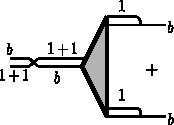
\includegraphics{inkscape/example1.pdf}
}
\end{center}

\begin{comment}
\jc{An additional ``problem'' is that since our circuits have a
left-to-right orientation, $A * B$ drawn as boxes left-to-right
gives an implicit ordering that is going to be hard to ignore.
I'm starting to think that the diagrams in the MO answer might
be better: use a colour (or like in Selinger's paper, at the
very end), symbols in the nodes that split.  So both would
be displayed as vertical stacks (only). Because I think that
swap* is too hard to justify in this notation. Of course,
if we could do things in 3D and $*$ was displayed using
(say) depth, that would be different again.}

This idea leads to a resource-based interpretation of types as
\emph{possible events} and of the values as \emph{consistent timelines
  of events} as explained below. The event $1$ is trivial, and the
event $0$ is impossible.  We visualize the denotation of $1$ as a
point in space, and $0$ as empty space. The denotation of $A + B$ is
the denotation of~$A$ drawn on top of the denotation of $B$ and
separated by a border, and the denotation of $A * B$ is just the
denotation of $A$ written next to the denotation of $B$.  For example,
let $2$ be the type $1 + 1$ represented by a stack of two boxes each
with a point inside it. The type $(2 + 2) * (2 + 2)$ would then be two
such stacks laid next to each other. Composing further, the type
$((2 + 2) * (2 + 2)) + ((2 + 2) * (2 + 2))$ is built by stacking the
last two diagrams as shown below on the left:
\begin{center}
\hfill
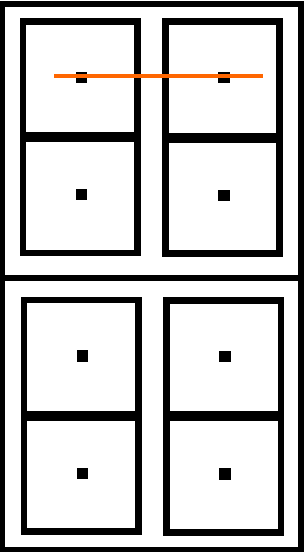
\includegraphics[scale=0.3]{images/tall-tl-1}
~
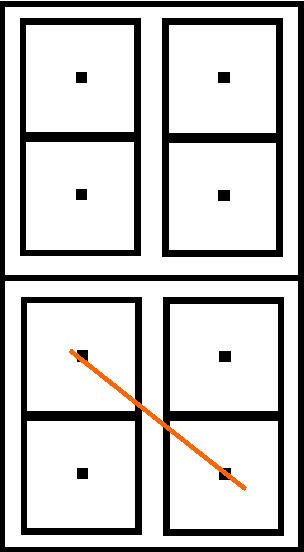
\includegraphics[scale=0.3]{images/tall-tl-2}
\hfill (*)
\end{center}
If we call the type on the left $A$ then the full diagram above
represents the type $A*A$.

To understand how diagrams (types) can transform through the
evaluation of  a program, we need to reason about the equivalence of
different diagrams. Consider for example, the two diagrams below:

\begin{center}
\hfill
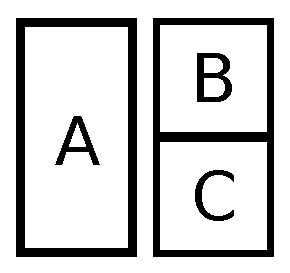
\includegraphics[scale=0.3]{images/distrib-1}
\qquad \qquad \qquad \qquad \qquad
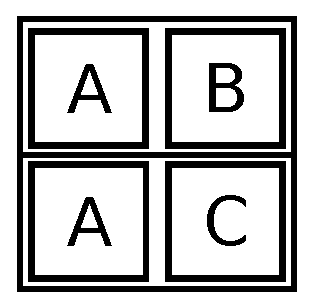
\includegraphics[scale=0.3]{images/distrib-2}
\hfill (**)
\end{center}

The diagram on the left represents the type $A * (B + C)$ while the
one on the right represents the type $(A * B) + (A * C)$. These two
types are equivalent in $\Pi$ but why are they equivalent in the
graphical notation? We argue that they admit the same consistent
timelines where a consistent timeline is defined recursively on the
structure of a diagram:
\begin{itemize}
\item An endpoint (the denotation of $1$) has exactly one timeline
  through it.  Empty space (the denotation of $0$) has no timelines
  through it.
\item A timeline through a stack of alternatives
  $A_1 + A_2 + \cdots + A_n$ is a timeline through exactly one of the
  possible alternatives.
\item A timeline through a spatial composition of cells
  $A_1 * A_2 * \cdots * A_n$ is a timeline through \emph{all} of the
  cells, in some order.
\end{itemize}

For example, the red line in the diagram (*) represents a consistent
timeline. For the diagrams (**), we note that any consistent timeline
for the left diagram must go through $A$ and either one of $B$ or $C$
and for the diagram on the right, the choice happens earlier but the
result is the same: any consistent timeline must go through either $A$
and $B$ or through $A$ and $C$.

Other than distributity, $\Pi$ combinators simply allow us to shuffle
the components of a stack around as well as shuffle the positions of
components in the plane.
\end{comment}
% \amr{
%   Let’s have a geometric representation of spaces:
% - A + B means putting A next to B
% - A * B means putting A and B on two perpendicular axes and filling
% the square (volume) between them
% All the combinators would indeed have a natural action and if we have
% a few nice pictures it would be great. What do you think? }

% \newcommand{\graphzero}{}
% \newcommand{\graphone}{\ensuremath{\bullet}}
% \newcommand{\graphplus}[2]{\node (top) {#1}; \node [below of=top] {#2};}

% \begin{center}
% \begin{tikzpicture} %% [declare function = {plus(\x,\y) = \node (top){\x}; \node [below of=top] {\y};}]
% \node (x) {\graphone};
% \node (y) {\graphone};
% %% {plus(\x,\y)}
% \end{tikzpicture}
% \end{center}

% \begin{definition}{Primitive operators of ~\ensuremath{\Pi } }
% \label{def:primitives-langRev}

% \[\begin{array}{rrcll}
%  \identlp :& 0 + b &\leftrightarrow & b &: \identrp \\
%  \swapp :& b_1 + b_2 &\leftrightarrow & b_2 + b_1 &: \swapp \\
%  \assoclp :& b_1 + (b_2 + b_3) &\leftrightarrow & (b_1 + b_2) + b_3 &: \assocrp \\
%  \identlt :& 1 \times b &\leftrightarrow & b &: \identrt \\
%  \swapt :& b_1 \times b_2 &\leftrightarrow & b_2 \times b_1 &: \swapt \\
%  \assoclt :& b_1 \times (b_2 \times b_3) &\leftrightarrow & (b_1 \times b_2) \times b_3 &: \assocrt \\
%  \absorbr :& 0 \times b &\leftrightarrow & 0 &: \factorzl \\
%  \dist :& (b_1 + b_2) \times b_3 &\leftrightarrow & (b_1 \times b_3) + (b_2 \times b_3) &: \factor \\
%  \end{array}\]
% %subcode source isomorphisms.tex:427

% \end{definition}


% Each line of this table is to be read as the definition of one or two
% operators. For example, corresponding to the \textit{identity of
%   \ensuremath{\times}} isomorphism (\ensuremath{1\times b\leftrightarrow b}) we have the two operators
% \ensuremath{\identlt:1\times b\leftrightarrow b} (reading the isomorphism from left to right) and
% \ensuremath{\identrt:b\leftrightarrow 1\times b} (reading the isomorphism from right to
% left). These operators are inverses of each other.  Each of the two
% cases of commutativity defines one operator that is its own inverse.

% Having defined primitive operators, we need some means of composing
% them. We construct the composition combinators out of the closure
% conditions for isomorphisms.

% \begin{definition}{Composition in \ensuremath{\Pi } }
% $$
% \infer{ \idc : b \leftrightarrow b}{
% 	 ~
% }
% \quad
% \infer{ \ !~c : b_2 \leftrightarrow b_1}{
% 	 c : b_1 \leftrightarrow b_2
% }
% \quad
% \infer{ c_1\odot c_2 : b_1 \leftrightarrow b_3}{
% 	 c_1 : b_1 \leftrightarrow b_2
% 	&
% 	 c_2 : b_2 \leftrightarrow b_3
% }
% $$
% $$
% \infer{ c_1 + c_2 : b_1 + b_2 \leftrightarrow b_3 + b_4}{
% 	 c_1 : b_1 \leftrightarrow b_3
% 	&
% 	 c_2 : b_2 \leftrightarrow b_4
% }
% \quad
% \infer{ c_1 \times c_2 : b_1 \times b_2 \leftrightarrow b_3 \times b_4}{
% 	 c_1 : b_1 \leftrightarrow b_3
% 	&
% 	 c_2 : b_2 \leftrightarrow b_4
% }
% $$
% %subcode source isomorphisms.tex:462
% \end{definition}

% Thus we have program constructs that witness reflexivity \ensuremath{\idc},
% symmetry \ensuremath{\mathit{sym}}, and transitivity~\ensuremath{\odot} and two parallel
% composition combinators, one for sums~\ensuremath{+} and one for
% pairs~\ensuremath{\times}.

%%%%%%%%%
\subsection{Denotational Semantics}

Figure~\ref{type-isos} introduces our desired denotational
semantices, and section~\ref{sec:opsem} a direct definition
of an operational semantics. One obvious question arises:
do these correspond? 

We can certainly associate to each $\Pi$ combinator an
equivalence between the denotation of each type%
\footnote{This is extracted from the Agda formalization
of this work, which has been reported on in~\cite{Carette2016}.}:
\begin{code}\hspace*{-4mm}
\>\AgdaFunction{c2equiv} \AgdaSymbol{:} \AgdaSymbol{\{}\AgdaBound{t₁}
\AgdaBound{t₂} \AgdaSymbol{:} \AgdaDatatype{U}\AgdaSymbol{\}} \AgdaSymbol{→}
\AgdaSymbol{(}\AgdaBound{c} \AgdaSymbol{:} \AgdaBound{t₁} \AgdaDatatype{⟷}
\AgdaBound{t₂}\AgdaSymbol{)} \AgdaSymbol{→} \AgdaFunction{⟦} \AgdaBound{t₁}
\AgdaFunction{⟧} \AgdaFunction{≃} \AgdaFunction{⟦} \AgdaBound{t₂}
\AgdaFunction{⟧}%
\end{code}

\noindent And as such an equivalence contains a function as
its first component, we can compare if our operational
semantics and denotational semantics match.  And they do:
\begin{code}\hspace*{-4mm}
\>\AgdaFunction{lemma0} \AgdaSymbol{:} \<[10]%
\>[10]\AgdaSymbol{\{}\AgdaBound{t₁} \AgdaBound{t₂} \AgdaSymbol{:}
\AgdaDatatype{U}\AgdaSymbol{\}} \AgdaSymbol{→} \AgdaSymbol{(}\AgdaBound{c}
\AgdaSymbol{:} \AgdaBound{t₁} \AgdaDatatype{⟷} \AgdaBound{t₂}\AgdaSymbol{)}
\AgdaSymbol{→} \AgdaSymbol{(}\AgdaBound{v} \AgdaSymbol{:} \AgdaFunction{⟦}
\AgdaBound{t₁} \AgdaFunction{⟧}\AgdaSymbol{)} \AgdaSymbol{→}
\AgdaFunction{eval} \AgdaBound{c} \AgdaBound{v} \AgdaDatatype{≡}
\AgdaField{proj₁} \AgdaSymbol{(}\AgdaFunction{c2equiv}
\AgdaBound{c}\AgdaSymbol{)} \AgdaBound{v}\<%
\end{code}

\noindent We can similarly hand-write a backwards evaluator,
prove that it is indeed a proper backwards evaluator, and
finally show that it agrees with the reverse equivalence.

%%%%%%%%%
\subsection{Examples}

Surprising expressiveness of Pi:

\begin{quote}
  Ed Fredkin pursued the idea that information must be finite in
  density. One day, he announced that things must be even more simple
  than that. He said that he was going to assume that information
  itself is conserved. “You’re out of you mind, Ed.” I
  pronounced. “That’s completely ridiculous. Nothing could happen in
  such a world. There couldn’t even be logical gates. No decisions
  could ever be made.” But when Fredkin gets one of his ideas, he’s
  quite immune to objections like that; indeed, they fuel him with
  energy. Soon he went on to assume that information processing must
  also be reversible — and invented what’s now called the Fredkin
  gate. (Minsky 1999)
\end{quote}

\begin{verbatim}
examples:
  (1 + 1) x ((1 + 1) x b) = (b+b) + (b+b)
  conditionals
  toffoli
  fredkin
  revisit adder example from Sec 2
  perhaps a larger example as well (from RC 18 paper?)
\end{verbatim}

\label{sec:langRev-examples}

In this section we introduce programming in \ensuremath{\Pi } through
several simple examples. We subsequently discuss the expressiveness of
the language and discuss various properties.

\label{examples}

\paragraph*{Booleans}
Let us start with encoding booleans. We use the type \ensuremath{1+1} to
represent booleans with \ensuremath{\mathit{left} ~()} representing \ensuremath{\mathit{true}} and
\ensuremath{\mathit{right}~()} representing \ensuremath{\mathit{false}}.
Boolean negation is straightforward to define:

\ensuremath{\mathit{not} : \mathit{bool} \leftrightarrow \mathit{bool}}

\ensuremath{\mathit{not} = \swapp}

\noindent
It is easy to verify that \ensuremath{\mathit{not}} changes \ensuremath{\mathit{true}} to \ensuremath{\mathit{false}} and
vice versa.

\paragraph*{Bit Vectors.}
We can represent $n$-bit words using an n-ary product of
\ensuremath{\mathit{bool}}s. For example, we can represent a 3-bit word, \ensuremath{\mathit{word}_3},
using the type \ensuremath{\mathit{bool}\times (\mathit{bool}\times \mathit{bool})}.  We can perform various
operations on these 3-bit words using combinators in \ensuremath{\Pi }. For
instance the bitwise \ensuremath{\mathit{not}} operation is the parallel composition of
three \ensuremath{\mathit{not}} operations:

\ensuremath{\mathit{not}_{\mathit{word}_3} :: \mathit{word}_3 \leftrightarrow \mathit{word}_3}

\ensuremath{\mathit{not}_{\mathit{word}_3} = \mathit{not} \times (\mathit{not} \times \mathit{not})}

\noindent We can express a 3-bit word reversal operation as follows:

\ensuremath{\mathit{reverse} : \mathit{word}_3 \leftrightarrow \mathit{word}_3}

\ensuremath{\mathit{reverse} = \swapt \odot (\swapt \times \idc)~ \odot \assocrt}

\noindent We can check that \ensuremath{\mathit{reverse}} does the right thing by
applying it to a value \ensuremath{(v_1, (v_2, v_3))} and writing out the full
derivation tree of the reduction.  The combinator \ensuremath{\mathit{reverse}}, like
many others we will see in this thesis, is formed by sequentially
composing several simpler combinators. Instead of presenting the
operation of \ensuremath{\mathit{reverse}} as a derivation tree, it is easier (purely
for presentation reasons) to flatten the tree into a sequence of
reductions as caused by each component. Such a sequence of reductions
is given below:
\[\begin{array}{rlr}
 & (v_1, (v_2, v_3)) \\
 \swapt & ((v_2, v_3), v_1) \\
 \swapt \times \idc & ((v_3, v_2), v_1) \\
 \assocrt & (v_3, (v_2, v_1)) \\
 \end{array}\]
%subcode source isomorphisms.tex:979

\noindent On the first line is the initial value. On each subsequent
line is a fragment of the \ensuremath{\mathit{reverse}} combinator and the value that
results from applying this combinator to the value on the previous
line. For example, \ensuremath{\swapt} transforms \ensuremath{(v_1, (v_2, v_3))} to
\ensuremath{((v_2,v_3),v_1)}.  On the last line we see the expected result with
the bits in reverse order.

We can also draw out the graphical representation of the 3-bit reverse
combinator. In the graphical representation, it is clear that the
combinator achieves the required shuffling.

\inkscape{reverse-3-bit.pdf}

\paragraph*{Conditionals.}
Even though \ensuremath{\Pi } lacks conditional expressions, they are
expressible using the distributivity and factoring laws. The
diagrammatic representation of \ensuremath{\dist} shows that it redirects the flow
of a value \ensuremath{v:b} based on the value of another one of type
\ensuremath{b_1+b_2}. If we choose \ensuremath{1+1} to be
\ensuremath{\mathit{bool}} and apply either \ensuremath{c_1:b_1\leftrightarrow
b_2} or \ensuremath{c_2:b_1\leftrightarrow b_2} to the value \ensuremath{v},
then we essentially have an `if' expression.

\ensuremath{\mathit{if}_{c_1,c_2} : \mathit{bool} \times b_1 \leftrightarrow \mathit{bool} \times b_2}

\ensuremath{\mathit{if}_{c_1,c_2} = \dist \odot ((\idc \times c_1) + (\idc \times c_2)) \odot \factor}


\inkscape{if-c1-c2.pdf}


The diagram above shows the input value of type \ensuremath{(1+1)\times b_2}
processed by the distribute operator \ensuremath{\dist}, which converts it into
a value of type \ensuremath{(1\times b_2)+(1\times b_2)}. In the
\ensuremath{\mathit{left}} branch, which corresponds to the
case when the boolean is \ensuremath{\mathit{true}} (i.e. the value was
\ensuremath{\mathit{left} ~()}), the combinator~\ensuremath{c_1} is applied to
the value of type~\ensuremath{b_1}. The right
branch which corresponds to the boolean being \ensuremath{\mathit{false}} passes
the value of type \ensuremath{b_1} through the combinator \ensuremath{c_2}.

\paragraph*{Logic Gates}
There are several universal primitives for conventional (irreversible)
hardware circuits, such as \ensuremath{\mathit{nand}} and \ensuremath{\mathit{fanout}}. In the case
of reversible hardware circuits, the canonical universal primitive is
the Toffoli gate~\cite{toffoli:1980}. The Toffoli gate takes three
boolean inputs: if the first two inputs are \ensuremath{\mathit{true}} then the third
bit is negated. In a traditional language, the Toffoli gate would be
most conveniently expressed as a conditional expression like:

\noindent
\ensuremath{ \mathit{toffoli}(v_1,v_2,v_3) = \mathit{if} ~(v_1 ~\mathit{and} ~v_2) ~\mathit{then} ~(v_1, v_2, \mathit{not}(v_3)) ~\mathit{else} ~(v_1, v_2, v_3)}

We will derive Toffoli gate in \ensuremath{\Pi } by first deriving a simpler
logic gate called \ensuremath{\mathit{cnot}}.  Consider a one-armed version, \ensuremath{\mathit{if}_c},
of the conditional derived above. If the \ensuremath{\mathit{bool}} is
\ensuremath{\mathit{true}}, the value of type \ensuremath{b} is modified by the operator \ensuremath{c}.

\begin{center}
\scalebox{1.5}{
%%subcode-line{pdfimage}[diagrams/if_c.pdf]
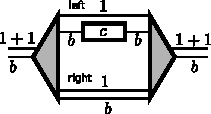
\includegraphics{inkscape/cnot.pdf}
}
\end{center}


By choosing \ensuremath{b} to be \ensuremath{\mathit{bool}} and \ensuremath{c} to be \ensuremath{\mathit{not}}, we have the
combinator \ensuremath{\mathit{if}_{\mathit{not}} : \mathit{bool}\times \mathit{bool}\leftrightarrow \mathit{bool}\times \mathit{bool}} which negates its
second argument if the first argument is \ensuremath{\mathit{true}}. This gate
\ensuremath{\mathit{if}_{\mathit{not}}} is often referred to as the \ensuremath{\mathit{cnot}} gate\cite{toffoli:1980}.

If we iterate this construction once more, the resulting combinator
\ensuremath{\mathit{if}_{\mathit{cnot}}} has type \ensuremath{\mathit{bool}\times (\mathit{bool}\times \mathit{bool})\leftrightarrow \mathit{bool}\times (\mathit{bool}\times \mathit{bool})}. The
resulting gate checks the first argument and if it is \ensuremath{\mathit{true}},
proceeds to check the second argument. If that is also \ensuremath{\mathit{true}} then
it will negate the third argument. Thus \ensuremath{\mathit{if}_{\mathit{cnot}}} is the required
Toffoli gate.

\begin{center}
\scalebox{1.6}{
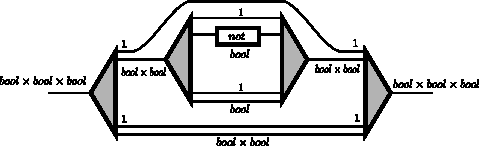
\includegraphics{inkscape/toffoli.pdf}
}
\end{center}

%%%%%%%%%%%%%%%%%%%%%%%%%%%%%%%%%%%%%%%%%%%%%%%%%%%%%%%%%%%%%%%%%
\section{Data III: Reversible Programs between Reversible Programs}
\label{sec:pi2}

In the previous sections, we examined equivalences between
conventional data structures, i.e., sets of values and structured trees
of values. We now consider a richer but
foundational notion of data: programs themselves. Indeed, universal
computation models crucially rely on the fact that \emph{programs
are (or can be encoded as) data}, e.g., a Turing machine can be
encoded as a string that another Turing machine (or even the same
machine) can manipulate. Similarly, first-class functions are
the \emph{only} values in the $\lambda$-calculus.
In our setting, the programs developed in the
previous section are reversible deformations between structured finite
types. We now ask whether these programs can themselves
be subject to (higher-level) reversible deformations?

Before developing the theory, let's consider a small example
consisting of two deformations between the types $A + B$ and $C+D$:

\begin{center}
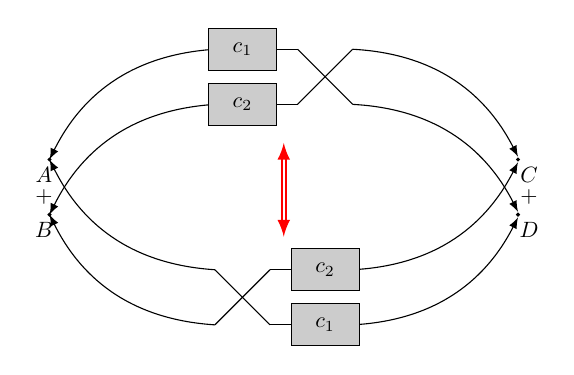
\begin{tikzpicture}[scale=0.7,every node/.style={scale=0.8}]
  \draw[>=latex,<->,double,red,thick] (2.25,-1.2) -- (2.25,-2.9) ;
%%  \node at (3.3,-2) {$\mathit{swapl}_{+\Leftrightarrow}$} ;
%%  \node at (2.5,-1.3) {$((c_2~\oplus~c_1)~\odot~\mathit{swap}_{+})$};
%%  \node at (2.5,-2.7) {$(\mathit{swap}_{+}~\odot~(c_1~\oplus~c_2))$};
%  \draw (-2,-2) ellipse (0.5cm and 1cm);
  \draw[fill] (-2,-1.5) circle [radius=0.025];
  \node[below] at (-2.1,-1.5) {$A$};
  \node[below] at (-2.1,-1.9) {$+$};
  \draw[fill] (-2,-2.5) circle [radius=0.025];
  \node[below] at (-2.1,-2.5) {$B$};

%  \draw (6.5,-2) ellipse (0.5cm and 1cm);
  \draw[fill] (6.5,-1.5) circle [radius=0.025];
  \node[below] at (6.7,-1.5) {$C$};
  \node[below] at (6.7,-1.9) {$+$};
  \draw[fill] (6.5,-2.5) circle [radius=0.025];
  \node[below] at (6.7,-2.5) {$D$};

  \draw[<-] (-2,-1.5) to[bend left] (1,0.5) ;
  \draw[<-] (-2,-2.5) to[bend left] (1,-0.5) ;
  \draw[->] (3.5,0.5) to[bend left] (6.5,-1.45) ;
  \draw[->] (3.5,-0.5) to[bend left] (6.5,-2.45) ;

  \draw[<-] (-2,-1.5) to[bend right] (1,-3.5) ;
  \draw[<-] (-2,-2.5) to[bend right] (1,-4.5) ;
  \draw[->] (3.5,-3.5) to[bend right] (6.5,-1.55) ;
  \draw[->] (3.5,-4.5) to[bend right] (6.5,-2.55) ;


  \draw     (2,0.5)  -- (2.5,0.5)  ;
  \draw     (2,-0.5) -- (2.5,-0.5) ;

  \draw     (2.5,0.5)  -- (3.5,-0.5)  ;
  \draw     (2.5,-0.5) -- (3.5,0.5) ;

  \draw     (1,-3.5)  -- (2,-4.5)    ;
  \draw     (1,-4.5) -- (2,-3.5)   ;

  \draw     (2,-3.5)  -- (2.5,-3.5)    ;
  \draw     (2,-4.5) -- (2.5,-4.5)   ;

  \path (1.5,0.5) node (tc1) [func] {$c_1$};
  %\draw     (1,0.9)  -- (2,0.9) -- (2,0.1) -- (1,0.1) -- cycle ;
  %\node at (1.5,0.5) {$c_1$};

  \path (1.5,-0.5) node (tc2) [func] {$c_2$};
  %\draw     (1,-0.1)  -- (2,-0.1) -- (2,-0.9) -- (1,-0.9) -- cycle ;
  %\node at (1.5,-0.5) {$c_2$};

  \path (3,-4.5) node (bc1) [func] {$c_1$};
  %\draw     (2.5,-4.1)  -- (3.5,-4.1) -- (3.5,-4.9) -- (2.5,-4.9) -- cycle ;
  %\node at (3,-4.5) {$c_1$};

  \path (3,-3.5) node (bc2) [func] {$c_2$};
  %\draw     (2.5,-3.1)  -- (3.5,-3.1) -- (3.5,-3.9) -- (2.5,-3.9) -- cycle ;
  % \node at (3,-3.5) {$c_2$};

\end{tikzpicture}
\end{center}
The top path is the $\Pi$ program
$(c_1~\oplus~c_2)~\odot~\swapp$ which deforms the
type $A$ by $c_1$, deforms the type $B$ by $c_2$, and deforms the
resulting space by a twist that exchanges the two injections into the
sum type. The bottom path performs the twist first and then deforms
the type $A$ by $c_1$ and the type $B$ by $c_2$ as before. One
could imagine the paths are physical \emph{elastic} wires in $3$ space, where
the deformations $c_1$ and $c_2$ as arbitrary deformations on these wires, and
the twists do not touch but are in fact well-separated. Then, holding the
points $A$, $B$, $C$, and $D$ fixed, it is possible to imagine
sliding $c_1$ and $c_2$ from the top wire rightward past the
twist, and then using the elasticity of the wires, pull the
twist back to line up with that of the bottom --- thus making
both parts of the diagram identical.  Each of these moves
can be undone (reversed), and doing so would take the bottom
part of the diagram into the top part.  In other
words, there exists a deformation of the program
$(c_1~\oplus~c_2)~\odot~\swapp$ to the program
$\swapp \odot (c_2~\oplus~c_1)$. We can also show that this
means that, as permutations, $(c_1~\oplus~c_2)~\odot~\swapp$ and
$\swapp \odot (c_2~\oplus~c_1)$ are equal. And, of course, not
all programs between the same types can be deformed into one
another. The simplest example of inequivalent deformations
are the two automorphisms of $1+1$, namely $\idc$ and $\swapp$.

While we will not make the details of the stretchable wires and
slidable boxes formal, it is useful for intuition.  One caveat
though: some of the sliding and stretching needs to be done in
spaces of higher dimension than 3 to have ``enough room'' to
move things along without collision or over-stretching wires.
That, unfortunately, means that some equivalences are harder to
grasp. Luckily, most equivalences only need 3 dimensions.

Our reversible language of type isomorphisms and equivalences between
them has a strong connection to \emph{univalent universes} in
HoTT~\cite{Carette2018}. Based on this connection, we refer to the
types as being at level-0, to the equivalences between types (i.e., the
combinators of Sec.~\ref{sec:pi1}) as being at level-1, and to the
equivalences between equivalences of types (i.e., the combinators
discussed in this section) as being at level-2.

%%%%%%%%%
\subsection{A Model of Equivalences between Type Equivalences}

Previously we saw how we could take the proof terms of commutative semirings
equivalences as our starting point for $\Pi$. What we need
now is to understand how \emph{proofs} of algebraic identities should be
considered equivalent. Classical algebra does not help, as proofs
are not considered first-class citizens. However,
another route is available to us: since the work of
Hofmann and Streicher~\cite{hofmann96thegroupoid}, we know that
one can model types as \emph{groupoids}.  The additional
structure comes from explicitly modeling the ``identity
types'': instead of regarding all terms which witness
the equality of (say) $a$ and $b$ of type $A$ as being
indistinguishable, we posit that there may in fact be many.
This consequences of this one decision are enough to show that
types can be modeled by groupoids.

Thus, rather than looking at (untyped) commutative semirings,
we should look at a \emph{typed} version. This process frequently
goes by the moniker of ``categorification.''  We want a categorical
algebra, where the basic objects are groupoids (to model our types),
and where there is a natural notion of $+$ and $*$.  At first,
we hit what seems like a serious stumbling block: the category of
all groupoids, \Gpd, does not have either co-products
nor products. However, we don't want to work internally in
\Gpd -- we want operations
\emph{on} groupoids. In other words, we want something akin to
symmetric monoidal categories, but with two interacting
monoidal structures.  Luckily, this already exists: the categorical
analog to (commutative) semirings are (symmetric) Rig
Categories~\cite{laplaza72,kelly74}.
This straightforwardly generalizes to symmetric Rig Groupoids.

How does this help? Coherence conditions! Symmetric monoidal categories,
to start somewhere simple, do not just introduce natural transformations
like the associator $\alpha$ and the left and right unitors ($\lambda$
and $\rho$ respectively), but also coherence conditions that these must satisfy.
Looking, for example, at just the additive fragment of $\Pi$ (i.e. with just $0$,
$1$ and $+$ for the types, $\odot$ and $\oplus$ as combinators, and
only the terms so expressible), the sub-language would correspond,
denotationally, to exactly (non-empty) symmetric monoidal groupoids. And what
these possess are exactly some \emph{equations between equations}
as commutative diagrams.  Transporting these coherence conditions, for
example those that express that various transformations are \emph{natural}
to $\Pi$, gives a list of equations between $\Pi$ programs.
Furthermore, all the natural transformations
that arise are in fact natural \emph{isomorphisms} -- and thus
reversible.

We can then proceed to prove that every one of the coherence conditions
involved in defining a symmetric Rig Groupoid holds for the groupoid
interpretation of types~\cite{Carette2016}.  This is somewhat tedious
given the sheer number of these, but when properly formulated,
relatively straightforward, but see below for comments on some
tricky cases.

But why are these particular coherence laws? Are they all necessary?
Conversely are they, in some appropriate sense, sufficient? This is
the so-called \emph{coherence problem}. Mac Lane, in his farewell address
as President of the American Mathematical Society~\cite{MacLane1976} gives
a good introduction and overview of such problems.  A more modern
interpretation (which can nevertheless be read into Mac Lane's own
exposition) would read as follows: given a set of equalities on abstract
words, regarded as a rewrite system, and two means of rewriting a word
in that language to another, is there some suitable notion of canonical
form that expresses the essential uniqueness of the non-trivial
rewrites?  Note how this word-and-rewrite problem is essentially
independent of the eventual interpretation. But one must take some care,
as there are obvious degenerate cases (involving ``trivial'' equations
involving $0$ or $1$) which lead to non-uniqueness. The landmark
results, first by Kelly-Mac Lane~\cite{KELLY197197} for closed
symmetric monoidal categories, then (independently) Laplaza and
Kelly~\cite{laplaza72,kelly74} for symmetric Rig Categories, is
that indeed there are sound and complete coherence conditions that
insure that all the ``obvious'' equalities between different abstract
words in these systems give rise to commutative diagrams. The
``obvious'' equalities come from \emph{syzygies} or
\emph{critical pairs} of the system of equations.

%%%%%%%%%
\subsection{A Language of Equivalences between Type Equivalences}
\label{langeqeq}

As motivated in the previous section, the equivalences between type
equivalences are perfectly modeled by the coherence conditions of weak
Rig Groupoids. Syntactically, we take the easiest way there: simply
make every coherence isomorphism into a programming construct. These
constructs are collected in several figures (Fig.~\ref{figj} to
Fig.~\ref{figa}) and are discussed next.

Conveniently, the various coherence conditions can be naturally
grouped into ``related'' laws.  Each group basically captures the
interactions between compositions of level-1 $\Pi$ combinators.

\begin{figure}[t]
Let $c_1 : t_1 \leftrightarrow t_2$, $c_2 : t_3 \leftrightarrow t_4$, $c_3 : t_1 \leftrightarrow t_2$, and $c_4 : t_3 \leftrightarrow t_4$. \\
Let $a_1 : t_5 \leftrightarrow t_1$,  $a_2 : t_6 \leftrightarrow t_2$, $a_3 : t_1 \leftrightarrow t_3$, and $a_4 : t_2 \leftrightarrow t_4$.
\[\def\arraystretch{1.3}
\begin{array}{c}
\Rule{}
  {c_1 \Leftrightarrow c_3 \quad c_2 \Leftrightarrow c_4}
  {c_1 \oplus c_2 \Leftrightarrow c_3 \oplus c_4}
  {}
\qquad
\Rule{}
  {c_1 \Leftrightarrow c_3 \quad c_2 \Leftrightarrow c_4}
  {c_1 \otimes c_2 \Leftrightarrow c_3 \otimes c_4}
  {}
\\
  {(a_1 \odot a_3) \oplus (a_2 \odot a_4) \Leftrightarrow (a_1 \oplus a_2) \odot (a_3 \oplus a_4)}
\\
  {(a_1 \odot a_3) \otimes (a_2 \odot a_4) \Leftrightarrow (a_1 \otimes a_2) \odot (a_3 \otimes a_4)}
\end{array}\]
\caption{\label{fige}Signatures of level-2 $\Pi$-combinators: functors}
\end{figure}

Starting with the simplest constructions, the first two constructs in
Fig.~\ref{fige} are the level-2 analogs of $+$ and $*$, which respectively
model combinator-level choice composition and parallel composition (of
equivalences).  These allow us to ``build up'' larger equivalences from smaller
ones.  The next two express that both of these composition operators distribute
over sequential composition $\odot$ (and vice versa).

\begin{figure}[t]
Let $c_1 : t_1 \leftrightarrow t_2$,  $c_2 : t_2 \leftrightarrow t_3$, and $c_3 : t_3 \leftrightarrow t_4$:
\[\def\arraystretch{1.3}
\begin{array}{c}
  {c_1 \odot (c_2 \odot c_3) \Leftrightarrow (c_1 \odot c_2) \odot c_3}
\\
  {(c_1 \oplus (c_2 \oplus c_3)) \odot \assoclp \Leftrightarrow \assoclp \odot ((c_1 \oplus c_2) \oplus c_3)}
\\
  {(c_1 \otimes (c_2 \otimes c_3)) \odot \assoclt \Leftrightarrow \assoclt \odot ((c_1 \otimes c_2) \otimes c_3)}
\\
  {((c_1 \oplus c_2) \oplus c_3) \odot \assocrp \Leftrightarrow \assocrp \odot (c_1 \oplus (c_2 \oplus c_3))}
\\
  {((c_1 \otimes c_2) \otimes c_3) \odot \assocrt \Leftrightarrow \assocrt \odot (c_1 \otimes (c_2 \otimes c_3))}
\\
  {\assocrp \odot \assocrp \Leftrightarrow ((\assocrp \oplus \idc) \odot \assocrp) \odot (\idc \oplus \assocrp)}
\\
  {\assocrt \odot \assocrt \Leftrightarrow ((\assocrt \otimes \idc) \odot \assocrt) \odot (\idc \otimes \assocrt)}
\end{array}\]
\caption{\label{figj}Signatures of level-2 $\Pi$-combinators: associativity}
\end{figure}

The constructs in Fig.~\ref{figj} capture the informal idea that all
the different ways of associating programs are equivalent. The first
says that sequential composition itself ($\odot$) is associative.
The next $4$ capture how
the $\oplus$ and $\otimes$ combinators ``commute'' with re-association.
In other words, it expresses the type-level associativity of $+$ is
properly reflected by the properties of $\oplus$.
The last two equivalences show how composition of associativity combinators
interact together. 
\begin{comment}
For example, the last equivalence captures the idea that the
program $\assocrt \odot \assocrt$ transforms an input of
type $((t_1 * t_2) * t_3) * t_4$ to an output of type
$t_1 * (t_2 * (t_3 * t_4))$ as follows:

\begin{center}
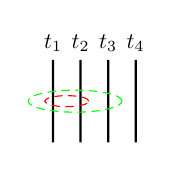
\begin{tikzpicture}[scale=0.7,every node/.style={scale=0.8},baseline=(current bounding box.center)]
\node[above] (A) at (-2,0) {$t_1$};
\node[above] (B) at (-1.5,0) {$t_2$};
\node[above] (C) at (-1,0) {$t_3$};
\node[above] (D) at (-0.5,0) {$t_4$};
\draw[thick] (A) -- (-2,-1.5);
\draw[thick] (B) -- (-1.5,-1.5);
\draw[thick] (C) -- (-1,-1.5);;
\draw[thick] (D) -- (-0.5,-1.5);
\draw[red,densely dashed] (-1.75,-0.75) ellipse [x radius=0.4cm, y radius = 0.1cm];
\draw[green,densely dashed] (-1.6,-0.75) ellipse [x radius=0.85cm, y radius = 0.2cm];
\end{tikzpicture}
$\leadsto$
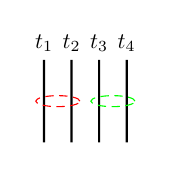
\begin{tikzpicture}[scale=0.7,every node/.style={scale=0.8},baseline=(current bounding box.center)]
\node[above] (A) at (-2,0) {$t_1$};
\node[above] (B) at (-1.5,0) {$t_2$};
\node[above] (C) at (-1,0) {$t_3$};
\node[above] (D) at (-0.5,0) {$t_4$};
\draw[thick] (A) -- (-2,-1.5);
\draw[thick] (B) -- (-1.5,-1.5);
\draw[thick] (C) -- (-1,-1.5);;
\draw[thick] (D) -- (-0.5,-1.5);
\draw[red,densely dashed] (-1.75,-0.75) ellipse [x radius=0.4cm, y radius = 0.1cm];
\draw[green,densely dashed] (-0.75,-0.75) ellipse [x radius=0.4cm, y radius = 0.1cm];
\end{tikzpicture}
$\leadsto$
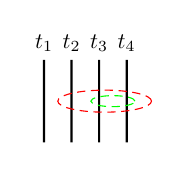
\begin{tikzpicture}[scale=0.7,every node/.style={scale=0.8},baseline=(current bounding box.center)]
\node[above] (A) at (-2,0) {$t_1$};
\node[above] (B) at (-1.5,0) {$t_2$};
\node[above] (C) at (-1,0) {$t_3$};
\node[above] (D) at (-0.5,0) {$t_4$};
\draw[thick] (A) -- (-2,-1.5);
\draw[thick] (B) -- (-1.5,-1.5);
\draw[thick] (C) -- (-1,-1.5);;
\draw[thick] (D) -- (-0.5,-1.5);
\draw[red,densely dashed] (-0.9,-0.75) ellipse [x radius=0.85cm, y radius = 0.2cm];
\draw[green,densely dashed] (-0.75,-0.75) ellipse [x radius=0.4cm, y radius = 0.1cm];
\end{tikzpicture}
\end{center}
% \[
% ((t_1 * t_2) * t_3) * t_4 \leadsto
% (t_1 * t_2) * (t_3 * t_4) \leadsto
% t_1 * (t_2 * (t_3 * t_4))
% \]

\noindent The program on the right
$((\assocrt \otimes \idc) \odot \assocrt) \odot (\idc \otimes
\assocrt)$ achieves the same end-to-end transformation using the
following sequence of steps:

\begin{center}
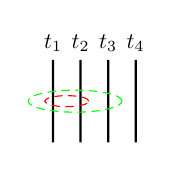
\begin{tikzpicture}[scale=0.7,every node/.style={scale=0.8},baseline=(current bounding box.center)]]
\node[above] (A) at (-2,0) {$t_1$};
\node[above] (B) at (-1.5,0) {$t_2$};
\node[above] (C) at (-1,0) {$t_3$};
\node[above] (D) at (-0.5,0) {$t_4$};
\draw[thick] (A) -- (-2,-1.5);
\draw[thick] (B) -- (-1.5,-1.5);
\draw[thick] (C) -- (-1,-1.5);;
\draw[thick] (D) -- (-0.5,-1.5);
\draw[red,densely dashed] (-1.75,-0.75) ellipse [x radius=0.4cm, y radius = 0.1cm];
\draw[green,densely dashed] (-1.6,-0.75) ellipse [x radius=0.85cm, y radius = 0.2cm];
\end{tikzpicture}
$\leadsto$
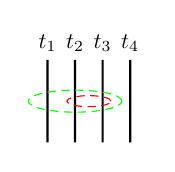
\begin{tikzpicture}[scale=0.7,every node/.style={scale=0.8},baseline=(current bounding box.center)]]
\node[above] (A) at (-2,0) {$t_1$};
\node[above] (B) at (-1.5,0) {$t_2$};
\node[above] (C) at (-1,0) {$t_3$};
\node[above] (D) at (-0.5,0) {$t_4$};
\draw[thick] (A) -- (-2,-1.5);
\draw[thick] (B) -- (-1.5,-1.5);
\draw[thick] (C) -- (-1,-1.5);;
\draw[thick] (D) -- (-0.5,-1.5);
\draw[red,densely dashed] (-1.25,-0.75) ellipse [x radius=0.4cm, y radius = 0.1cm];
\draw[green,densely dashed] (-1.5,-0.75) ellipse [x radius=0.85cm, y radius = 0.2cm];
\end{tikzpicture}
$\leadsto$
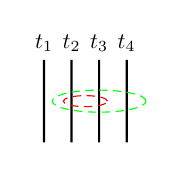
\begin{tikzpicture}[scale=0.7,every node/.style={scale=0.8},baseline=(current bounding box.center)]]
\node[above] (A) at (-2,0) {$t_1$};
\node[above] (B) at (-1.5,0) {$t_2$};
\node[above] (C) at (-1,0) {$t_3$};
\node[above] (D) at (-0.5,0) {$t_4$};
\draw[thick] (A) -- (-2,-1.5);
\draw[thick] (B) -- (-1.5,-1.5);
\draw[thick] (C) -- (-1,-1.5);;
\draw[thick] (D) -- (-0.5,-1.5);
\draw[red,densely dashed] (-1.25,-0.75) ellipse [x radius=0.4cm, y radius = 0.1cm];
\draw[green,densely dashed] (-1.0,-0.75) ellipse [x radius=0.85cm, y radius = 0.2cm];
\end{tikzpicture}
$\leadsto$
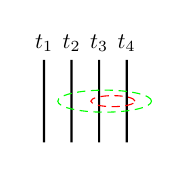
\begin{tikzpicture}[scale=0.7,every node/.style={scale=0.8},baseline=(current bounding box.center)]]
\node[above] (A) at (-2,0) {$t_1$};
\node[above] (B) at (-1.5,0) {$t_2$};
\node[above] (C) at (-1,0) {$t_3$};
\node[above] (D) at (-0.5,0) {$t_4$};
\draw[thick] (A) -- (-2,-1.5);
\draw[thick] (B) -- (-1.5,-1.5);
\draw[thick] (C) -- (-1,-1.5);;
\draw[thick] (D) -- (-0.5,-1.5);
\draw[green,densely dashed] (-0.9,-0.75) ellipse [x radius=0.85cm, y radius = 0.2cm];
\draw[red,densely dashed] (-0.75,-0.75) ellipse [x radius=0.4cm, y radius = 0.1cm];
\end{tikzpicture}
\end{center}
% \[
% ((t_1 * t_2) * t_3) * t_4 \leadsto
% (t_1 * (t_2 * t_3)) * t_4 \leadsto
% t_1 * ((t_2 * t_3) * t_4) \leadsto
% t_1 * (t_2 * (t_3 * t_4))
% \]

\jc{I am not a big fan of these pictures -- mainly because I can't give any
intuition based on them of why these can be smoothly deformed into one another.
All the ``pictures'' I can come up with [via purely formal reasoning] sit in at least
5 dimensions -- one for each of the wires, and another to give room to maneuver.}
\end{comment}

\jc{need to find some combinators whose diagrams can help illustrate 
the ideas further. Enough so that the next paragraph makes sense.}

\noindent This of course gives rise to a \emph{critical pair} in words over the
level-1 language, as both of these programs are between the same types.
Since neither of these involve either trivial types (like $0$ or $1$) nor
twists (i.e. automorphisms) on the types themselves, coherence requires that
these in fact be equivalent programs.  One interpretation is that
\emph{outermost} re-associations is the same as \emph{innermost}
re-associations.

\begin{figure}[t]
Let $c_1 : t_1 \leftrightarrow t_2$, $c_2 : t_3 \leftrightarrow t_4$, and $c_3 : t_5 \leftrightarrow t_6$:
\[\def\arraystretch{1.3}
\begin{array}{c}
  {((c_1 \oplus c_2) \otimes c_3) \odot \dist \Leftrightarrow \dist \odot ((c_1 \otimes c_3) \oplus (c_2 \otimes c_3))}
\\
  {(c_1 \otimes (c_2 \oplus c_3)) \odot \distl \Leftrightarrow \distl \odot ((c_1 \otimes c_2) \oplus (c_1 \otimes c_3))}
\\
  {((c_1 \otimes c_3) \oplus (c_2 \otimes c_3)) \odot \factor \Leftrightarrow \factor \odot ((c_1 \oplus c_2) \otimes c_3)}
\\
  {((c_1 \otimes c_2) \oplus (c_1 \otimes c_3)) \odot \factorl \Leftrightarrow \factorl \odot (c_1 \otimes (c_2 \oplus c_3))}
\end{array}\]
\caption{\label{figi}Signatures of level-2 $\Pi$-combinators: distributivity and factoring}
\end{figure}

The constructs in Fig.~\ref{figi} are the basic coherence for
$\dist$, $\distl$, $\factor$ and $\factorl$: the type-level distribution
and factoring has to commute with the combinator-level $\oplus$ and $\otimes$.

\begin{comment}
\begin{center}
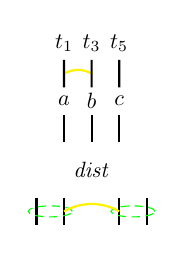
\begin{tikzpicture}[scale=0.7,every node/.style={scale=0.8}]
\node[above] (A) at (-2,0) {$t_1$};
\node[above] (B) at (-1.5,0) {$t_3$};
\node[above] (C) at (-1,0) {$t_5$};
\draw[thick,yellow] (-1.5,-0.25) arc[start angle=60, end angle=120, radius=0.5cm];
\draw[thick] (A) -- (-2,-0.5);
\draw[thick] (B) -- (-1.5,-0.5);
\draw[thick] (C) -- (-1,-0.5);
\node at (-2,-0.75) {$a$};
\node at (-1.5,-0.75) {$b$};
\node at (-1,-0.75) {$c$};
\draw[thick] (-2,-1) -- (-2,-1.5);
\draw[thick] (-1.5,-1) -- (-1.5,-1.5);
\draw[thick] (-1,-1) -- (-1,-1.5);
\node at (-1.5,-2) {$\dist$};
\draw[thick] (-2.5,-2.5) -- (-2.5,-3);
\draw[thick] (-2,-2.5) -- (-2,-3);
\draw[green,densely dashed] (-2.25,-2.75) ellipse [x radius=0.4cm, y radius = 0.1cm];
\draw[thick] (-1,-2.5) -- (-1,-3);
\draw[thick] (-0.5,-2.5) -- (-0.5,-3);
\draw[green,densely dashed] (-0.75,-2.75) ellipse [x radius=0.4cm, y radius = 0.1cm];
\draw[thick,yellow] (-1,-2.75) arc[start angle=60, end angle=120, radius=1cm];
\end{tikzpicture}
\end{center}
% ((a + b) * c) ; dist <=> dist ; ((a * c) + (b * c))
% LHS: (t1 + t3) * t5 ~> (t2 + t4) * t6 ~> (t2 * t6) + (t4 * t6)
% RHS: (t1 + t3) * t5 ~> (t1 * t5) + (t3 * t5) ~> (t2 * t6) + (t4 * t6)
\end{comment}

\begin{figure}[t]
Let $c_0, c_1, c_2, c_3 : t_1 \leftrightarrow t_2$ and $c_4, c_5 : t_3 \leftrightarrow t_4$:
\[\def\arraystretch{1.3}
\begin{array}{c}
  {\idc \odot \, c_0 \Leftrightarrow c_0}
\quad
  {c_0 \, \odot \idc \, \Leftrightarrow c_0}
\quad
  {c_0\,\, \odot\,!\, c_0 \Leftrightarrow \idc}
\quad
  {!\, c_0 \odot c_0 \Leftrightarrow \idc}
\\
  {\idc \oplus \, \idc \, \Leftrightarrow \idc}
\qquad
  {\idc \otimes \, \idc \, \Leftrightarrow \idc}
\\
  {c_0 \Leftrightarrow c_0}
\quad
\Rule{}
  {c_1 \Leftrightarrow c_2 \quad c_2 \Leftrightarrow c_3}
  {c_1 \Leftrightarrow c_3}
  {}
\quad
\Rule{}
  {c_1 \Leftrightarrow c_4 \quad c_2 \Leftrightarrow c_5}
  {c_1 \odot c_2 \Leftrightarrow c_4 \odot c_5}
  {}
\end{array}\]
\caption{\label{figh}Signatures of level-2 $\Pi$-combinators: identity and composition}
\end{figure}

The constructs in Fig.~\ref{figh} express various properties of composition.
The first two says that $\idc$ is a left and right identity for sequential composition.
The next two say that all programs are reversible, both on the left and the right:
running $c$ and then its reverse ($!\, c$) is equivalent to the identity, and the
same for doing $!\, c$ first then $c$. The last line say that there is an
identity level-2 combinator, a sequential composition, and that level-2
equivalence respects level-1 sequential composition $\odot$.

\begin{figure}[t]
Let $c_0 : 0 \leftrightarrow 0$, $c_1 : 1 \leftrightarrow 1$, and $c_3 : t_1 \leftrightarrow t_2$:
\[\def\arraystretch{1.3}
\begin{array}{c}
  {\identlp \odot c_3 \Leftrightarrow (c_0 \oplus c_3) \odot \identlp}
\qquad
  {\identrp \odot (c_0 \oplus c_3) \Leftrightarrow c_3 \odot \identrp}
\\
  {\identlsp \odot c_3 \Leftrightarrow (c_3 \oplus c_0) \odot \identlsp}
\qquad
  {\identrsp \odot (c_3 \oplus c_0) \Leftrightarrow c_3 \odot \identrsp}
\\
  {\identlt \odot c_3 \Leftrightarrow (c_1 \otimes c_3) \odot \identlt}
\qquad
  {\identrt \odot (c_1 \otimes c_3) \Leftrightarrow c_3 \odot \identrp}
\\
  {\identlst \odot c_3 \Leftrightarrow (c_3 \otimes c_1) \odot \identlst}
\qquad
  {\identrst \odot (c_3 \otimes c_1) \Leftrightarrow c_3 \odot \identrst}
\\
  {\identlt \Leftrightarrow \distl \odot (\identlt \oplus \identlt)}
\\
\identlp \Leftrightarrow \swapp \odot \identlsp
\qquad
\identlt \Leftrightarrow \swapt \odot \identlst
\end{array}\]
\caption{\label{figg}Signatures of level-2 $\Pi$-combinators: unit}
\end{figure}

The constructs in Fig.~\ref{figg} may at first blush look similarly straightforward,
but deserve some pause. One obvious question: What is the point of
$c_0 : 0 \leftrightarrow 0$, isn't that just the identity combinator $\idc$
for $A = 0$ (as defined in Fig.~\ref{type-isos})? Operationally, $c_0$
is indeed indistinguishable from $\idc$. However, there are multiple syntactic
ways of writing down combinators of type $0 \leftrightarrow 0$, and the
first combinator in Fig.~\ref{figg} applies to all of them uniformly.
This is another subtle aspect of coherence: all reasoning must be valid for
all possible models, not just the one we have in mind. So even though
operational reasoning may suggest that some relations \emph{may} be
true between combinators, it can also mislead. The same reasoning
applies to $c_1 : 1 \leftrightarrow 1$.  The first $8$ combinators can
then be read as basic coherence for unit introduction and elimination,
in both additive and multiplicative cases.

The last two capture
another simple idea, related to swapping: eliminating a unit
on the left is the same as first swapping then eliminating on the
right (both additively and multiplicatively). As a side note,
these are not related to \emph{commutativity}, but rather
come from one of the simplest coherence condition for
braided monoidal categories. In other words, it reflects the
idempotence of $\swapp$ and $\swapt$ rather than the
commutativity of $\oplus$ and $\otimes$.

\begin{figure}[t]
Let $c_1 : t_1 \leftrightarrow t_2$ and $c_2 : t_3 \leftrightarrow t_4$:
\[\def\arraystretch{1.3}
\begin{array}{c}
  {\swapp \odot (c_1 \oplus c_2) \Leftrightarrow (c_2 \oplus c_1) \odot \swapp}
\quad
  {\swapt \odot (c_1 \otimes c_2) \Leftrightarrow (c_2 \otimes c_1) \odot \swapt}
\\
  {(\assocrp \odot \swapp) \odot \assocrp \Leftrightarrow ((\swapp \oplus \idc) \odot \assocrp) \odot (\idc \oplus \swapp)}
\\
  {(\assoclp \odot \swapp) \odot \assoclp \Leftrightarrow ((\idc \oplus \swapp) \odot \assoclp) \odot (\swapp \oplus \idc)}
\\
  {(\assocrt \odot \swapt) \odot \assocrt \Leftrightarrow ((\swapt \otimes \idc) \odot \assocrt) \odot (\idc \otimes \swapt)}
\\
  {(\assoclt \odot \swapt) \odot \assoclt \Leftrightarrow ((\idc \otimes \swapt) \odot \assoclt) \odot (\swapt \otimes \idc)}
\end{array}\]
\caption{\label{figf}Signatures of level-2 $\Pi$-combinators: commutativity and associativity}
\end{figure}

The first two equivalences in Fig.~\ref{figf} reflect the basic
coherence between type-level swapping and and the level-2 combinator
actions. The next four arise because of interactions between
(additive and multiplicative) level-1 associativity and swapping.
In other words, they arise as critical pairs.  For example,
the first expresses that the two ways of going from
$\left(A \oplus B\right) \oplus C$ to $B \oplus \left(C \oplus A\right)$
are equivalent, with the second saying that the reverse (i.e.
the results of applying $!$\,) also gives equivalent programs.
The last two say the same but for the multiplicative structure.

\begin{figure}[t]
\[\def\arraystretch{1.3}
\begin{array}{c}
  {\identlsp \oplus \idc ~\Leftrightarrow~ \assocrp \odot (\idc \oplus \, \identlp)}
\\
  {\identlst \otimes \idc ~\Leftrightarrow~ \assocrt \odot (\idc \otimes \, \identlt)}
\end{array}\]
\caption{\label{figd}Signatures of level-2 $\Pi$-combinators: unit and associativity}
\end{figure}

The constructs in Fig.~\ref{figd} express how unit elimination ``in the middle''
can be expressed either as operating on the right or, (after re-association) on the left.


\begin{figure}[t]
Let $c : t_1 \leftrightarrow t_2$:
\[\def\arraystretch{1.3}
\begin{array}{c}
  {(c \otimes \idc) \odot \absorbl \Leftrightarrow \absorbl \odot \idc}
\quad
  {(\idc \, \otimes c) \odot \absorbr \Leftrightarrow \absorbr \odot \idc}
\\
  {\idc \odot \, \factorzl \Leftrightarrow \factorzl \odot (\idc \otimes c)}
\quad
  {\idc \odot \, \factorzr \Leftrightarrow \factorzr \odot (c \otimes \idc)}
\\
  {\absorbr \Leftrightarrow \absorbl}
\\
  {\absorbr \Leftrightarrow (\distl \odot (\absorbr \oplus \absorbr)) \odot \identlp}
\\
  {\identlst \Leftrightarrow \absorbr}
\qquad
  {\absorbl \Leftrightarrow \swapt \odot \absorbr}
\\
  {\absorbr \Leftrightarrow (\assoclt \odot (\absorbr \otimes \idc)) \odot \absorbr}
\\
  {(\idc \otimes \absorbr) \odot \absorbl \Leftrightarrow (\assoclt \odot (\absorbl \otimes \idc)) \odot \absorbr}
\\
  {\idc \otimes \, \identlp \Leftrightarrow (\distl \odot (\absorbl \oplus \idc)) \odot \identlp}
\end{array}\]
\caption{\label{figc}Signatures of level-2 $\Pi$-combinators: zero}
\end{figure}

The constructs in Fig.~\ref{figc} are significantly more subtle, as they
deal with combinators involving $0$, aka an impossibility.  For example,
\[  {(c \otimes \idc_{0}) \odot \absorbl \Leftrightarrow \absorbl \odot \idc_{0}}
\]
(where we have explicitly annotated the types of $\idc$ for increased clarity)
tells us that of the two ways of transforming from $t_1 \times 0$ to $0$, 
namely first doing some arbitrary transformation $c$ from $t_1$ to $t_2$ and
(in parallel) leaving $0$ alone then eliminating $0$, or first eliminating $0$
then doing the identity (at $0$), are equivalent. This is the ``naturality'' of
$\absorbl$. One item to note is the fact that this combinator is not
irreducible, as the $\idc$ on the right can be eliminated. But that is actually
a property visible at an even higher level (which we will not touch in this
paper).  The next $3$ are similarly expressing the naturality of $\absorbr$,
$\factorzl$ and $\factorzr$.

The next combinator, $\absorbr \Leftrightarrow \absorbl$,
is particularly fascinating: while it says something simple ---
that the two obvious ways of transforming $0 \times 0$ into $0$, namely
absorbing either the left or right zero --- it implies something subtle.
A straightforward proof of $\absorbl$ which proceeds by saying that
$0 \times t$ cannot be inhabited because the first member of the pair
cannot, is not in fact equivalent to $\absorbr$ on $0 \times 0$.
However, if we instead define $\absorbl$ to ``transport'' the
putative impossible first member of the pair to its (equally
impossible) output, then these do form equivalent pairs.
The next few in Fig.~\ref{figc} also express how $\absorbr$ and
$\absorbl$ interact with other combinators. As seen previously,
all of these arise as critical pairs. What is much more subtle here
is that the types involved often are asymmetric: they do not have
the same occurences on the left and right. Such cases are
particularly troublesome for finding normal forms \jc{should add
some citations here}.

\begin{figure}[t]
\[\def\arraystretch{1.3}
\begin{array}{c}
  {((\assoclp \otimes \idc) \odot \dist) \odot (\dist \oplus \idc) \Leftrightarrow (\dist \odot (\idc \oplus \dist)) \odot \assoclp}
\\
  {\assoclt \odot \distl \Leftrightarrow ((\idc \otimes \distl) \odot \distl) \odot (\assoclt \oplus \assoclt)}
\end{array}\]
\vspace{ -0.5em}
\[\def\arraystretch{1.3}
\begin{array}{rcl}
  (\distl \odot (\dist \oplus \dist)) \odot \assoclp &\Leftrightarrow&
   \dist \odot (\distl \oplus \distl) \odot \assoclp ~\odot \\
&& (\assocrp \oplus \idc) ~\odot \\
&& ((\idc \oplus \swapp) \oplus \idc) ~\odot \\
&&      (\assoclp \oplus \idc)
\end{array}\]
\caption{\label{figb}Signatures of level-2 $\Pi$-combinators: associativity and distributivity}
\end{figure}

\begin{figure}[t]
\[\def\arraystretch{1.3}
\begin{array}{rcl}
  (\idc \otimes \swapp) \odot \distl &\Leftrightarrow& \distl \odot \swapp
\\
  \dist \odot (\swapt \oplus \swapt) &\Leftrightarrow & \swapt \odot \distl
\end{array}\]
\caption{\label{figa}Signatures of level-2 $\Pi$-combinators: commutativity and distributivity}
\end{figure}

The constructs in Fig.~\ref{figb} and Fig.~\ref{figa} relating associativity and
distributivity, and commutativity and distributivity, have more in common with
previous sets of combinators.  They do arise from non-trivial critical pairs
of different ways of going between equivalent types. The last one of
Fig.~\ref{figb} is particularly daunting, involving a sequence of $3$ combinators
on the left and $6$ on the right.

%%%%%%%%%
\subsection{Operational Semantics}

We can do for the level-2 combinators the same as was done for level-1:
create a programming language with these combinators as fundamental
constants, typed by level-1 combinators. But we can do more, as these
new combinators are exactly rewrites for level-1 programs.  Thus,
it is possible to create

%%%%%%%%%
% \subsection{Graphical Language}
% 
% Idea: thinking in the 3D way; we have collections of towers of
% blocks. Every 1-combinator involves touching some blocks, swapping
% them around, etc. Two 1-combinators are equivalent if they touch the
% same blocks the same number of times. ??

%%%%%%%%%
\subsection{Examples}

We illustrate our methodology using a small example. Consider a
circuit that takes an input type consisting of three values
\Tree [ {\small a} [ {\small b} {\small c} ] ]~
and swaps the leftmost value with the rightmost value
to produce
\Tree [ {\small c} [ {\small b} {\small a} ] ]~.
We can implement two such circuits using our Agda library for $\Pi$:

\begin{code}%
\>[0]\AgdaFunction{swap{-}fl1}\AgdaSpace{}%
\AgdaFunction{swap{-}fl2}\AgdaSpace{}%
\AgdaSymbol{:}\AgdaSpace{}%
\AgdaSymbol{\{}\AgdaBound{a}\AgdaSpace{}%
\AgdaBound{b}\AgdaSpace{}%
\AgdaBound{c}\AgdaSpace{}%
\AgdaSymbol{:}\AgdaSpace{}%
\AgdaDatatype{U}\AgdaSymbol{\}}\AgdaSpace{}%
\AgdaSymbol{→}\AgdaSpace{}%
\AgdaInductiveConstructor{PLUS}\AgdaSpace{}%
\AgdaBound{a}\AgdaSpace{}%
\AgdaSymbol{(}\AgdaInductiveConstructor{PLUS}\AgdaSpace{}%
\AgdaBound{b}\AgdaSpace{}%
\AgdaBound{c}\AgdaSymbol{)}\AgdaSpace{}%
\AgdaDatatype{⟷}\AgdaSpace{}%
\AgdaInductiveConstructor{PLUS}\AgdaSpace{}%
\AgdaBound{c}\AgdaSpace{}%
\AgdaSymbol{(}\AgdaInductiveConstructor{PLUS}\AgdaSpace{}%
\AgdaBound{b}\AgdaSpace{}%
\AgdaBound{a}\AgdaSymbol{)}\<%
\\
\>[0]\AgdaFunction{swap{-}fl1}\AgdaSpace{}%
\AgdaSymbol{=}\AgdaSpace{}%
\AgdaInductiveConstructor{assocl₊}\AgdaSpace{}%
\AgdaInductiveConstructor{◎}\AgdaSpace{}%
\AgdaInductiveConstructor{swap₊}\AgdaSpace{}%
\AgdaInductiveConstructor{◎}\AgdaSpace{}%
\AgdaSymbol{(}\AgdaInductiveConstructor{id⟷}\AgdaSpace{}%
\AgdaInductiveConstructor{⊕}\AgdaSpace{}%
\AgdaInductiveConstructor{swap₊}\AgdaSymbol{)}\<%
\\
%
\\[\AgdaEmptyExtraSkip]%
\>[0]\AgdaFunction{swap{-}fl2}\AgdaSpace{}%
\AgdaSymbol{=}%
\>[52I]\AgdaSymbol{(}\AgdaInductiveConstructor{id⟷}\AgdaSpace{}%
\AgdaInductiveConstructor{⊕}\AgdaSpace{}%
\AgdaInductiveConstructor{swap₊}\AgdaSymbol{)}\AgdaSpace{}%
\AgdaInductiveConstructor{◎}\<%
\\
\>[.]\<[52I]%
\>[11]\AgdaInductiveConstructor{assocl₊}\AgdaSpace{}%
\AgdaInductiveConstructor{◎}\<%
\\
%
\>[11]\AgdaSymbol{(}\AgdaInductiveConstructor{swap₊}\AgdaSpace{}%
\AgdaInductiveConstructor{⊕}\AgdaSpace{}%
\AgdaInductiveConstructor{id⟷}\AgdaSymbol{)}\AgdaSpace{}%
\AgdaInductiveConstructor{◎}\<%
\\
%
\>[11]\AgdaInductiveConstructor{assocr₊}\AgdaSpace{}%
\AgdaInductiveConstructor{◎}\<%
\\
%
\>[11]\AgdaSymbol{(}\AgdaInductiveConstructor{id⟷}\AgdaSpace{}%
\AgdaInductiveConstructor{⊕}\AgdaSpace{}%
\AgdaInductiveConstructor{swap₊}\AgdaSymbol{)}\<%
\end{code}

\noindent The first implementation rewrites the incoming values as follows:
\[
\Tree [ {\small a} [ {\small b} {\small c} ] ] ~\to~
\Tree [ [ {\small a} {\small b} ] {\small c} ] ~\to~
\Tree [ {\small c} [ {\small a} {\small b} ] ] ~\to~
\Tree [ {\small c} [ {\small b} {\small a} ] ] ~.
\]
\noindent
The second implementation rewrites the incoming values as follows:
\[
\Tree [ {\small a} [ {\small b} {\small c} ] ] ~\to~
\Tree [ {\small a} [ {\small c} {\small b} ] ] ~\to~
\Tree [ [ {\small a} {\small c} ] {\small b} ] ~\to~
\Tree [ [ {\small c} {\small a} ] {\small b} ] ~\to~
\Tree [ {\small c} [ {\small a} {\small b} ] ] ~\to~
\Tree [ {\small c} [ {\small b} {\small a} ] ] ~.
\]
\noindent The two circuits are extensionally equal. Using the level-2
isomorphisms we can \emph{explicitly} construct a sequence of
rewriting steps that transforms the second circuit to the first.  The proof
can be read as follows: the first three lines ``refocus'' from a right-associated
isomorphism onto the (left-associated) composition of the first $3$ isomorphisms;
then apply a complex rewrite on these (the ``hexagon'' coherence condition
of symmetric braided monoidal categories); this exposes two inverse combinators
next to each other --- so we have to refocus on these to eliminate them; we
finally re-associate to get the result.

\renewcommand{\AgdaIndentSpace}{\;\;}
\setlength\mathindent{0.5em}

\begin{samepage}
\begin{code}%
\>[0]\AgdaFunction{swap{-}fl2⇔swap{-}fl1}\AgdaSpace{}%
\AgdaSymbol{:}\AgdaSpace{}%
\AgdaSymbol{\{}\AgdaBound{a}\AgdaSpace{}%
\AgdaBound{b}\AgdaSpace{}%
\AgdaBound{c}\AgdaSpace{}%
\AgdaSymbol{:}\AgdaSpace{}%
\AgdaDatatype{U}\AgdaSymbol{\}}\AgdaSpace{}%
\AgdaSymbol{→}\AgdaSpace{}%
\AgdaFunction{swap{-}fl2}\AgdaSpace{}%
\AgdaSymbol{\{}\AgdaBound{a}\AgdaSymbol{\}}\AgdaSpace{}%
\AgdaSymbol{\{}\AgdaBound{b}\AgdaSymbol{\}}\AgdaSpace{}%
\AgdaSymbol{\{}\AgdaBound{c}\AgdaSymbol{\}}\AgdaSpace{}%
\AgdaOperator{\AgdaDatatype{⇔}}\AgdaSpace{}%
\AgdaFunction{swap{-}fl1}\<%
\\
\>[0]\AgdaFunction{swap{-}fl2⇔swap{-}fl1}\AgdaSpace{}%
\AgdaSymbol{=}\<%
\\
\>[0][@{}l@{\AgdaIndent{0}}]%
\>[2]\AgdaSymbol{((}\AgdaInductiveConstructor{id⟷}\AgdaSpace{}%
\AgdaOperator{\AgdaInductiveConstructor{⊕}}\AgdaSpace{}%
\AgdaInductiveConstructor{swap₊}\AgdaSymbol{)}\AgdaSpace{}%
\AgdaOperator{\AgdaInductiveConstructor{◎}}\AgdaSpace{}%
\AgdaInductiveConstructor{assocl₊}\AgdaSpace{}%
\AgdaOperator{\AgdaInductiveConstructor{◎}}\AgdaSpace{}%
\AgdaSymbol{(}\AgdaInductiveConstructor{swap₊}\AgdaSpace{}%
\AgdaOperator{\AgdaInductiveConstructor{⊕}}\AgdaSpace{}%
\AgdaInductiveConstructor{id⟷}\AgdaSymbol{)}\AgdaSpace{}%
\AgdaOperator{\AgdaInductiveConstructor{◎}}\AgdaSpace{}%
\AgdaInductiveConstructor{assocr₊}\AgdaSpace{}%
\AgdaOperator{\AgdaInductiveConstructor{◎}}\AgdaSpace{}%
\AgdaSymbol{(}\AgdaInductiveConstructor{id⟷}\AgdaSpace{}%
\AgdaOperator{\AgdaInductiveConstructor{⊕}}\AgdaSpace{}%
\AgdaInductiveConstructor{swap₊}\AgdaSymbol{))}%
\>[75]\AgdaOperator{\AgdaFunction{⇔⟨}}\AgdaSpace{}%
\AgdaInductiveConstructor{id⇔}\AgdaSpace{}%
\AgdaOperator{\AgdaInductiveConstructor{⊡}}\AgdaSpace{}%
\AgdaInductiveConstructor{assoc◎l}\AgdaSpace{}%
\AgdaOperator{\AgdaFunction{⟩}}\<%
\\
%
\>[2]\AgdaSymbol{((}\AgdaInductiveConstructor{id⟷}\AgdaSpace{}%
\AgdaOperator{\AgdaInductiveConstructor{⊕}}\AgdaSpace{}%
\AgdaInductiveConstructor{swap₊}\AgdaSymbol{)}\AgdaSpace{}%
\AgdaOperator{\AgdaInductiveConstructor{◎}}\AgdaSpace{}%
\AgdaSymbol{(}\AgdaInductiveConstructor{assocl₊}\AgdaSpace{}%
\AgdaOperator{\AgdaInductiveConstructor{◎}}\AgdaSpace{}%
\AgdaSymbol{(}\AgdaInductiveConstructor{swap₊}\AgdaSpace{}%
\AgdaOperator{\AgdaInductiveConstructor{⊕}}\AgdaSpace{}%
\AgdaInductiveConstructor{id⟷}\AgdaSymbol{))}\AgdaSpace{}%
\AgdaOperator{\AgdaInductiveConstructor{◎}}\AgdaSpace{}%
\AgdaInductiveConstructor{assocr₊}\AgdaSpace{}%
\AgdaOperator{\AgdaInductiveConstructor{◎}}\AgdaSpace{}%
\AgdaSymbol{(}\AgdaInductiveConstructor{id⟷}\AgdaSpace{}%
\AgdaOperator{\AgdaInductiveConstructor{⊕}}\AgdaSpace{}%
\AgdaInductiveConstructor{swap₊}\AgdaSymbol{))}%
\>[75]\AgdaOperator{\AgdaFunction{⇔⟨}}\AgdaSpace{}%
\AgdaInductiveConstructor{assoc◎l}\AgdaSpace{}%
\AgdaOperator{\AgdaFunction{⟩}}\<%
\\
%
\>[2]\AgdaSymbol{(((}\AgdaInductiveConstructor{id⟷}\AgdaSpace{}%
\AgdaOperator{\AgdaInductiveConstructor{⊕}}\AgdaSpace{}%
\AgdaInductiveConstructor{swap₊}\AgdaSymbol{)}\AgdaSpace{}%
\AgdaOperator{\AgdaInductiveConstructor{◎}}\AgdaSpace{}%
\AgdaInductiveConstructor{assocl₊}\AgdaSpace{}%
\AgdaOperator{\AgdaInductiveConstructor{◎}}\AgdaSpace{}%
\AgdaSymbol{(}\AgdaInductiveConstructor{swap₊}\AgdaSpace{}%
\AgdaOperator{\AgdaInductiveConstructor{⊕}}\AgdaSpace{}%
\AgdaInductiveConstructor{id⟷}\AgdaSymbol{))}\AgdaSpace{}%
\AgdaOperator{\AgdaInductiveConstructor{◎}}\AgdaSpace{}%
\AgdaInductiveConstructor{assocr₊}\AgdaSpace{}%
\AgdaOperator{\AgdaInductiveConstructor{◎}}\AgdaSpace{}%
\AgdaSymbol{(}\AgdaInductiveConstructor{id⟷}\AgdaSpace{}%
\AgdaOperator{\AgdaInductiveConstructor{⊕}}\AgdaSpace{}%
\AgdaInductiveConstructor{swap₊}\AgdaSymbol{))}%
\>[75]\AgdaOperator{\AgdaFunction{⇔⟨}}\AgdaSpace{}%
\AgdaInductiveConstructor{assoc◎l}\AgdaSpace{}%
\AgdaOperator{\AgdaInductiveConstructor{⊡}}\AgdaSpace{}%
\AgdaInductiveConstructor{id⇔}\AgdaSpace{}%
\AgdaOperator{\AgdaFunction{⟩}}\<%
\\
%
\>[2]\AgdaSymbol{((((}\AgdaInductiveConstructor{id⟷}\AgdaSpace{}%
\AgdaOperator{\AgdaInductiveConstructor{⊕}}\AgdaSpace{}%
\AgdaInductiveConstructor{swap₊}\AgdaSymbol{)}\AgdaSpace{}%
\AgdaOperator{\AgdaInductiveConstructor{◎}}\AgdaSpace{}%
\AgdaInductiveConstructor{assocl₊}\AgdaSymbol{)}\AgdaSpace{}%
\AgdaOperator{\AgdaInductiveConstructor{◎}}\AgdaSpace{}%
\AgdaSymbol{(}\AgdaInductiveConstructor{swap₊}\AgdaSpace{}%
\AgdaOperator{\AgdaInductiveConstructor{⊕}}\AgdaSpace{}%
\AgdaInductiveConstructor{id⟷}\AgdaSymbol{))}\AgdaSpace{}%
\AgdaOperator{\AgdaInductiveConstructor{◎}}\AgdaSpace{}%
\AgdaInductiveConstructor{assocr₊}\AgdaSpace{}%
\AgdaOperator{\AgdaInductiveConstructor{◎}}\AgdaSpace{}%
\AgdaSymbol{(}\AgdaInductiveConstructor{id⟷}\AgdaSpace{}%
\AgdaOperator{\AgdaInductiveConstructor{⊕}}\AgdaSpace{}%
\AgdaInductiveConstructor{swap₊}\AgdaSymbol{))}%
\>[75]\AgdaOperator{\AgdaFunction{⇔⟨}}\AgdaSpace{}%
\AgdaInductiveConstructor{hexagonl⊕r}\AgdaSpace{}%
\AgdaOperator{\AgdaInductiveConstructor{⊡}}\AgdaSpace{}%
\AgdaInductiveConstructor{id⇔}\AgdaSpace{}%
\AgdaOperator{\AgdaFunction{⟩}}\<%
\\
%
\>[2]\AgdaSymbol{(((}\AgdaInductiveConstructor{assocl₊}\AgdaSpace{}%
\AgdaOperator{\AgdaInductiveConstructor{◎}}\AgdaSpace{}%
\AgdaInductiveConstructor{swap₊}\AgdaSymbol{)}\AgdaSpace{}%
\AgdaOperator{\AgdaInductiveConstructor{◎}}\AgdaSpace{}%
\AgdaInductiveConstructor{assocl₊}\AgdaSymbol{)}\AgdaSpace{}%
\AgdaOperator{\AgdaInductiveConstructor{◎}}\AgdaSpace{}%
\AgdaInductiveConstructor{assocr₊}%
\>[44]\AgdaOperator{\AgdaInductiveConstructor{◎}}\AgdaSpace{}%
\AgdaSymbol{(}\AgdaInductiveConstructor{id⟷}\AgdaSpace{}%
\AgdaOperator{\AgdaInductiveConstructor{⊕}}\AgdaSpace{}%
\AgdaInductiveConstructor{swap₊}\AgdaSymbol{))}%
\>[75]\AgdaOperator{\AgdaFunction{⇔⟨}}\AgdaSpace{}%
\AgdaInductiveConstructor{assoc◎r}\AgdaSpace{}%
\AgdaOperator{\AgdaFunction{⟩}}\<%
\\
%
\>[2]\AgdaSymbol{((}\AgdaInductiveConstructor{assocl₊}\AgdaSpace{}%
\AgdaOperator{\AgdaInductiveConstructor{◎}}\AgdaSpace{}%
\AgdaInductiveConstructor{swap₊}\AgdaSymbol{)}\AgdaSpace{}%
\AgdaOperator{\AgdaInductiveConstructor{◎}}\AgdaSpace{}%
\AgdaInductiveConstructor{assocl₊}\AgdaSpace{}%
\AgdaOperator{\AgdaInductiveConstructor{◎}}\AgdaSpace{}%
\AgdaInductiveConstructor{assocr₊}%
\>[42]\AgdaOperator{\AgdaInductiveConstructor{◎}}\AgdaSpace{}%
\AgdaSymbol{(}\AgdaInductiveConstructor{id⟷}\AgdaSpace{}%
\AgdaOperator{\AgdaInductiveConstructor{⊕}}\AgdaSpace{}%
\AgdaInductiveConstructor{swap₊}\AgdaSymbol{))}%
\>[75]\AgdaOperator{\AgdaFunction{⇔⟨}}\AgdaSpace{}%
\AgdaInductiveConstructor{id⇔}\AgdaSpace{}%
\AgdaOperator{\AgdaInductiveConstructor{⊡}}\AgdaSpace{}%
\AgdaInductiveConstructor{assoc◎l}\AgdaSpace{}%
\AgdaOperator{\AgdaFunction{⟩}}\<%
\\
%
\>[2]\AgdaSymbol{((}\AgdaInductiveConstructor{assocl₊}\AgdaSpace{}%
\AgdaOperator{\AgdaInductiveConstructor{◎}}\AgdaSpace{}%
\AgdaInductiveConstructor{swap₊}\AgdaSymbol{)}\AgdaSpace{}%
\AgdaOperator{\AgdaInductiveConstructor{◎}}\AgdaSpace{}%
\AgdaSymbol{(}\AgdaInductiveConstructor{assocl₊}\AgdaSpace{}%
\AgdaOperator{\AgdaInductiveConstructor{◎}}\AgdaSpace{}%
\AgdaInductiveConstructor{assocr₊}\AgdaSymbol{)}%
\>[44]\AgdaOperator{\AgdaInductiveConstructor{◎}}\AgdaSpace{}%
\AgdaSymbol{(}\AgdaInductiveConstructor{id⟷}\AgdaSpace{}%
\AgdaOperator{\AgdaInductiveConstructor{⊕}}\AgdaSpace{}%
\AgdaInductiveConstructor{swap₊}\AgdaSymbol{))}%
\>[75]\AgdaOperator{\AgdaFunction{⇔⟨}}\AgdaSpace{}%
\AgdaInductiveConstructor{id⇔}\AgdaSpace{}%
\AgdaOperator{\AgdaInductiveConstructor{⊡}}\AgdaSpace{}%
\AgdaSymbol{(}\AgdaInductiveConstructor{linv◎l}\AgdaSpace{}%
\AgdaOperator{\AgdaInductiveConstructor{⊡}}\AgdaSpace{}%
\AgdaInductiveConstructor{id⇔}\AgdaSymbol{)}\AgdaSpace{}%
\AgdaOperator{\AgdaFunction{⟩}}\<%
\\
%
\>[2]\AgdaSymbol{((}\AgdaInductiveConstructor{assocl₊}\AgdaSpace{}%
\AgdaOperator{\AgdaInductiveConstructor{◎}}\AgdaSpace{}%
\AgdaInductiveConstructor{swap₊}\AgdaSymbol{)}\AgdaSpace{}%
\AgdaOperator{\AgdaInductiveConstructor{◎}}\AgdaSpace{}%
\AgdaInductiveConstructor{id⟷}%
\>[28]\AgdaOperator{\AgdaInductiveConstructor{◎}}\AgdaSpace{}%
\AgdaSymbol{(}\AgdaInductiveConstructor{id⟷}\AgdaSpace{}%
\AgdaOperator{\AgdaInductiveConstructor{⊕}}\AgdaSpace{}%
\AgdaInductiveConstructor{swap₊}\AgdaSymbol{))}%
\>[75]\AgdaOperator{\AgdaFunction{⇔⟨}}\AgdaSpace{}%
\AgdaInductiveConstructor{id⇔}\AgdaSpace{}%
\AgdaOperator{\AgdaInductiveConstructor{⊡}}\AgdaSpace{}%
\AgdaInductiveConstructor{idl◎l}\AgdaSpace{}%
\AgdaOperator{\AgdaFunction{⟩}}\<%
\\
%
\>[2]\AgdaSymbol{((}\AgdaInductiveConstructor{assocl₊}\AgdaSpace{}%
\AgdaOperator{\AgdaInductiveConstructor{◎}}\AgdaSpace{}%
\AgdaInductiveConstructor{swap₊}\AgdaSymbol{)}%
\>[22]\AgdaOperator{\AgdaInductiveConstructor{◎}}\AgdaSpace{}%
\AgdaSymbol{(}\AgdaInductiveConstructor{id⟷}\AgdaSpace{}%
\AgdaOperator{\AgdaInductiveConstructor{⊕}}\AgdaSpace{}%
\AgdaInductiveConstructor{swap₊}\AgdaSymbol{))}%
\>[75]\AgdaOperator{\AgdaFunction{⇔⟨}}\AgdaSpace{}%
\AgdaInductiveConstructor{assoc◎r}\AgdaSpace{}%
\AgdaOperator{\AgdaFunction{⟩}}\<%
\\
%
\>[2]\AgdaSymbol{((}\AgdaInductiveConstructor{assocl₊}\AgdaSpace{}%
\AgdaOperator{\AgdaInductiveConstructor{◎}}\AgdaSpace{}%
\AgdaInductiveConstructor{swap₊}\AgdaSpace{}%
\AgdaOperator{\AgdaInductiveConstructor{◎}}\AgdaSpace{}%
\AgdaSymbol{(}\AgdaInductiveConstructor{id⟷}\AgdaSpace{}%
\AgdaOperator{\AgdaInductiveConstructor{⊕}}\AgdaSpace{}%
\AgdaInductiveConstructor{swap₊}\AgdaSymbol{))}\AgdaSpace{}%
\AgdaOperator{\AgdaFunction{▤}}\AgdaSymbol{)}\<%
\end{code}
\end{samepage}

\renewcommand{\AgdaIndentSpace}{\AgdaSpace{}$\;\;$}

%%%%%%%%%%%%%%%%%%%%%%%%%%%%%%%%%%%%%%%%%%%%%%%%%%%%%%%%%%%%%%%%%
\section{Further Thoughts and Conclusions}

We conclude with a collection of open problems and avenues for further research.

%%%
\subsection{Richer Data: Infinite Sets and Topological Spaces}

The three languages we discussed only deal with the finite spaces
built from 0, 1, sums, and products. Programming practice, logic, and
mathematics all deal with richer spaces including inductive types
(e.g., the natural numbers, sequences, and trees), functions, and
graphs. Extending $\Pi$ to such domains is possible but only after one
refines the notions of reversibility and conservation of
information. One approach is to use \emph{partial isomorphisms} that
may be undefined on such inputs~\cite{infeffects,rc2011}. Another more
speculative approach is to build such spaces, topologically, based on
novel type constructions such as negative, fractional, or even
imaginary types~\cite{seventrees,roshan-thesis}.

%%%
\subsection{Information Effects}

A computational model that enforces the principle of conservation of
information is arguably \emph{richer} than a conventional model that
cannot even express the notion of information. Practically the
conventional model is easily recovered by simply adding constructs
that intentionally and explicitly create or erase information. Such
constructs allow one to recover the classical perspective with the
added advantage that it is possible to reason about such creation and
erasure of information using type and effect systems, monads, or
arrows~\cite{infeffects,inversearrows}.

An interesting application of such an idea is in the field of
\emph{information-flow security}. To make this idea concrete, consider
a tiny 2-bit password = \verb|"10"| and the associated password checker:

\begin{verbatim}
check-password (guess) =
  guess == "10"
\end{verbatim}

One can ask how much information is leaked by this program assuming
the attacker has no prior knowledge except that the password is 2
bits, i.e., the four possible 2-bits are equally likely. If the
attacker guesses \verb|"10"| (with probability $1/4$) the password (2
bits) is leaked. If the attacker guesses one of the other choices
(with probability $3/4$) the number of possibilities is reduced from 4
to 3, i.e., the attacker learns $\log{4} - \log{3}$ bits of
information. So in general the attacker learns:
\[\begin{array}{ll}
   &  1/4 * 2 + 3/4 (\log{4} - \log{3}) \\
  =&  1/4 \log{4} + 3/4 \log{4/3} \\
  =&  - 1/4 \log{1/4} - 3/4 \log{3/4} \\
  \sim& 0.8 \mbox{~bits~in~the~first~probe}
\end{array}\]
This is a significant amount of information. But of course this is
only because the password is so short: if the password was 8
restricted ASCII characters (6 bits), the attacker would only learn
0.00001 bits in the first probe.

An alternative formulation of the problem is to view the input as a
random variable with 4 possibilities and a uniform distribution (i.e.,
with 2 bits of information) and the output as another random variable
with 4 possibilities but with the distribution
$\{ (\mathit{True}, 1/4), (\mathit{False}, 3/4) \}$ which contains 0.8 bits of
information. Thus 2 input bits of information were given to the
password checker and only 0.8 were produced. Where did the 1.2 bits of
information go? By the Landauer Principle, these 1.2 bits must be
accounted by an \emph{implicit} \emph{erasure} operation in the
program. By writing the password checker in an extension of $\Pi$, the
erasure construct becomes explicit and the information leak becomes
exposed in the syntactic structure of the program~\cite{infeffects}.

%%%
\subsection{Theseus and Quantum Control}

The $\Pi$ family of languages semantically captures the principles of
reversibility and conservation of information. As a programming
language it has some mixed properties: small programs are relatively
easy to write; for some special classes of programs, it is even
possible to define a methodology to write large $\Pi$ programs,
including a meta-circular interpreter for $\Pi$~\cite{isoint}. In
general, however, the point-free style of combinators used in $\Pi$
becomes awkward and a new approach appears more suitable. To that end,
we note that $\Pi$ encodes the most elementary control structure in a
programming language-- which is the ability to conditionally execute
one of several possible code fragments-- using combinators. Expressing
such an abstraction using combinators or even predicates and nested
\textbf{if}-expressions makes it difficult for both humans and
compilers to write, understand, and reason about the control flow
structure of the program. Instead, in modern functional languages,
this control flow paradigm is elegantly expressed using
\emph{pattern-matching}. This approach yields code that is not only
more concise and readable but also enables the compiler to easily
verify two crucial properties: (i) non-overlapping patterns and (ii)
exhaustive coverage of a datatype using a collection of
patterns. Indeed most compilers for functional languages perform these
checks, warning the user when they are violated. At a more fundamental
level, e.g., in type theories and proof assistants, these properties
are actually necessary for correct reasoning about programs. Our
insight is that these properties, perhaps surprisingly, are sufficient
to produce a simple and intuitive first-order reversible programming
language which we call \emph{Theseus}.

\begin{figure}[t]
  \centering
  \begin{minipage}{0.4\linewidth}
    \begin{verbatim}
f :: Either Int Int -> a
f (Left 0)     = undefined
f (Left (n+1)) = undefined
f (Right n)    = undefined
\end{verbatim}\vspace{-4ex}
    \caption{A skeleton}\label{fig:intro-ex-1}
  \end{minipage}
  \hfill
  \begin{minipage}{0.4\linewidth}
\begin{verbatim}
g :: (Bool,Int) -> a
g (False,n)  = undefined
g (True,0)   = undefined
g (True,n+1) = undefined
\end{verbatim}\vspace{-4ex}
    \caption{Another skeleton}\label{fig:intro-ex-2}
  \end{minipage}
  \\[3ex]
  \begin{minipage}{0.6\linewidth}
\begin{verbatim}
h :: Either Int Int <-> (Bool,Int)
h (Left 0)     = (True,0)
h (Left (n+1)) = (False,n)
h (Right n)    = (True,n+1)
\end{verbatim}\vspace{-4ex}
    \caption{An isomorphism}\label{fig:intro-ex-3}
  \end{minipage}
\end{figure}

We provide a small illustrative example, written in a Haskell-like
syntax.  Fig.~\ref{fig:intro-ex-1} gives the skeleton of a function
\verb|f| that accepts a value of type \verb|Either Int| \verb|Int|;
the patterns on the left-hand side exhaustively cover every possible
incoming value and are non-overlapping. Similarly,
Fig.~\ref{fig:intro-ex-2} gives the skeleton for a function~\verb|g|
that accepts a value of type \verb|(Bool,Int)|; again the patterns on
the left-hand side exhaustively cover every possible incoming value
and are non-overlapping. Now we claim that since the types
\verb|Either Int Int| and \verb|(Bool,Int)| are isomorphic, we can
combine the patterns of \verb|f| and \verb|g| into \emph{symmetric
  pattern-matching clauses} to produce a reversible function between
the types \verb|Either Int Int| and
\verb|(Bool,Int)|. Fig.~\ref{fig:intro-ex-3} gives one such function;
there, we suggestively use \verb|<->| to indicate that the function
can be executed in either direction. This reversible function is
obtained by simply combining the non-overlapping exhaustive patterns
on the two sides of a clause. In order to be well-formed in either
direction, these clauses are subject to the constraint that each
variable occurring on one side must occur exactly once on the other
side (and with the same type). Thus it is acceptable to swap the
second and third right-hand sides of \verb|h| but not the first and
second ones. With some additional work, it is possible to extend
Theseus to a full-fledged reversible programming
language~\cite{theseus}. With just one additional insight, Theseus can
be extended with superpositions and becomes a quantum programming
language~\cite{10.1007/978-3-319-89366-2_19}.

%%%
\subsection{Summary}

The entire edifice of computer science including its mainstream models
of computations, programming languages, and logics is founded on
\emph{classical physics.} While much of the world phenomena can be
approximated with classical physics, we are reaching a revolutionary
period of quantum technology that challenges many of the classical
assumptions. It remains to be seen how computer science will adapt to
this quantum revolution but we believe that additional physical
principles inspired by quantum mechanics will have to be embraced in
our computational thinking. This paper focused on one such principle
--- \emph{conservation of information} --- and explored some of its
exciting implications to the field of computer science.

%%%%%%%%%%%%%%%%%%%%%%%%%%%%%%%%%%%%%%%%%%%%%%%%%%%%%%%%%%%%%%%%%
\section*{Acknowledgements} We would like to thank the numerous
students and colleagues who participated in various aspects of this
research and who provided valuable feedback and constructive criticism.

\bibliographystyle{unsrt}
\bibliography{cites}
\end{document}

%%%%%%%%%%%%%%%%%%%%%%%%%%%%%%%%%%%%%%%%%%%%%%%%%%%%%%%%%%%%%%%%%
%%%%%%%%%%%%%%%%%%%%%%%%%%%%%%%%%%%%%%%%%%%%%%%%%%%%%%%%%%%%%%%%%





\begin{comment}
\section{Theseus: Types and Simple Isomorphisms}
\label{theseusI}

We begin by presenting the core of Theseus which consists of evidently
reversible functions on user-defined datatypes.  In subsequent discourse we
will use the word `map' to refer to these logically reversible
functions. Theseus has the same built-in types as~\ensuremath{\Pi^{o}} and as conventional
functional programming languages: the empty type, the unit type, and sum and
product types. All other types, including recursive types, are user-defined
using a general mechanism for type declarations:

\lstset{
        language=haskell,
 morekeywords={Bool,Nat,Tree},
	keywordstyle=\bfseries\ttfamily,
	identifierstyle=\ttfamily,
	commentstyle=\ttfamily,
	stringstyle=\ttfamily,
	showstringspaces=false,
	basicstyle=\scriptsize\sffamily,
	tabsize=2,
	breaklines=false,
	breakatwhitespace=false,
	aboveskip={1.2\baselineskip},
        columns=fixed,
        extendedchars=true,
}
\begin{lstlisting}[escapeinside={(@}{@)}]
type Bool  =  (@\ctr{True}@) | (@\ctr{False}@)
type Nat   =  0 | Succ Nat
type Tree  =  Leaf Nat | Node Tree Tree
 \end{lstlisting}
%subcode source theseus.tex:347

\noindent The declarations above witness isomorphisms between the set
\kw{Bool} and the set constructed by the constants \ctr{True} and
\ctr{False}, between the set \kw{Nat} and the set inductively constructed
using {\scriptsize{0}} and \ctr{Succ}, and between the set \kw{Tree} and the
set inductively constructed using \ctr{Leaf} and \ctr{Node}.  Thus, Theseus
type definitions are similar to, say, Haskell, type definitions. Such
definitions translate directly to the underlying \ensuremath{\Pi^{o}} using iso-recursive
type definitions. For example, the above types translate as follows:
\vspace{-20pt}
\begin{small}
\begin{multicols}{3}
\[\begin{array}{rclr}
\kw{Bool}   & = &  \mu  ~x.1 + 1 \\
\kw{Nat}   & = &  \mu  ~x. 1 + x \\
\kw{Tree}   & = &  \mu  ~x. \kw{Nat}  + x * x \\
 \end{array}\]
%subcode source theseus.tex:363

\[\begin{array}{rclr}
\mathit{unfoldBool} :& \kw{Bool}  \leftrightarrow 1 + 1 &: \mathit{foldBool} \\
\mathit{unfoldNat} :& \kw{Nat}  \leftrightarrow 1 + \kw{Nat}  &: \mathit{foldNat} \\
\mathit{unfoldTree} :& \kw{Tree}  \leftrightarrow \kw{Nat}  + (\kw{Tree}  * \kw{Tree} ) &: \mathit{foldTree} \\
 \end{array}\]
%subcode source theseus.tex:368
\end{multicols}
\end{small}

%%%%%%%%%%%%
\subsection{Simple Isomorphisms}

A Theseus program has a type of the form \ctr{a} $\leftrightarrow$ \ctr{b};
one runs such a program forward by supplying a value of type \ctr{a}. If the
program terminates, we get back a value of type~\ctr{b}. Alternately we can
run the program in reverse by supplying a value of type \ctr{b}. Given the
built-in types and the facility to introduce user-defined ones, one can
already write a few small but interesting programs. Maps that are evidently
isomorphisms can be written in the familiar pattern matching style
popularized by the family of functional languages. For example:
\begin{multicols}{2}
\lstset{
        language=haskell,
 morekeywords={Nat,Tree,Int,Bool},
	keywordstyle=\bfseries\ttfamily,
	identifierstyle=\ttfamily,
	commentstyle=\ttfamily,
	stringstyle=\ttfamily,
	showstringspaces=false,
	basicstyle=\scriptsize\sffamily,
	tabsize=2,
	breaklines=false,
	breakatwhitespace=false,
	aboveskip={1.2\baselineskip},
        columns=fixed,
        extendedchars=true,
}
\begin{lstlisting}[escapeinside={(@}{@)}]
(@\ctr{id}@) :: Bool (@$\leftrightarrow$@) Bool
| (@\ctr{False}@)  (@$\leftrightarrow$@)  (@\ctr{False}@)
| (@\ctr{True}@)   (@$\leftrightarrow$@)  (@\ctr{True}@)

expandBool :: Bool * a (@$\leftrightarrow$@) a + a
| (@\ctr{True}@), a   (@$\leftrightarrow$@)  (@\ctr{Left}@) a
| (@\ctr{False}@), a  (@$\leftrightarrow$@)  (@\ctr{Right}@) a

expandNat :: Nat (@$\leftrightarrow$@) Nat + 1
| 0       (@$\leftrightarrow$@)  (@\ctr{Right}@) ()
| Succ n  (@$\leftrightarrow$@)  (@\ctr{Left}@) n

(@\ctr{not}@) :: Bool (@$\leftrightarrow$@) Bool
| (@\ctr{True}@)   (@$\leftrightarrow$@)  (@\ctr{False}@)
| (@\ctr{False}@)  (@$\leftrightarrow$@)  (@\ctr{True}@)

foldBool :: a + a (@$\leftrightarrow$@) Bool * a
| (@\ctr{Left}@) a   (@$\leftrightarrow$@)  (@\ctr{True}@), a
| (@\ctr{Right}@) a  (@$\leftrightarrow$@)  (@\ctr{False}@), a

foldNat :: Nat + 1 (@$\leftrightarrow$@) Nat
| (@\ctr{Right}@) ()  (@$\leftrightarrow$@)  0
| (@\ctr{Left}@) n    (@$\leftrightarrow$@)  Succ n
 \end{lstlisting}
%subcode source theseus.tex:410
\end{multicols}

\vspace{-25pt}
\lstset{
        language=haskell,
 morekeywords={Nat,Tree,Int,Bool},
	keywordstyle=\bfseries\ttfamily,
	identifierstyle=\ttfamily,
	commentstyle=\ttfamily,
	stringstyle=\ttfamily,
	showstringspaces=false,
	basicstyle=\scriptsize\sffamily,
	tabsize=2,
	breaklines=false,
	breakatwhitespace=false,
	aboveskip={1.2\baselineskip},
        columns=fixed,
        extendedchars=true,
}
\begin{lstlisting}[escapeinside={(@}{@)}]
treeUnwind :: Tree (@$\leftrightarrow$@) Tree * Tree + (Bool + Nat)
| Node t1 t2            (@$\leftrightarrow$@)  (@\ctr{Left}@)   (t1, t2)
| Leaf 0                (@$\leftrightarrow$@)  (@\ctr{Right}@)  ((@\ctr{Left}@) (@\ctr{True}@))
| Leaf (Succ 0)         (@$\leftrightarrow$@)  (@\ctr{Right}@)  ((@\ctr{Left}@) (@\ctr{False}@))
| Leaf (Succ (Succ n))  (@$\leftrightarrow$@)  (@\ctr{Right}@)  ((@\ctr{Right}@) n)
 \end{lstlisting}
%subcode source theseus.tex:422

Unlike the situation in a conventional functional language, the
intuition here is that the two sides of each pattern clause can be
swapped to produce the inverse of the function, i.e. as we will see
repeatedly in the paper, patterns and expressions are the same
thing. Compare for example the definitions of \ctr{expandBool} and
\ctr{foldBool}. This is the only constraint that a programmer needs to
maintain. This constraint can be ensured using the following two
rules:

\begin{enumerate}
\label{rules}
\item \emph{Non-overlapping and exhaustive coverage in pattern
  clauses.} The collections of patterns in the left-hand side (LHS) of
  each clause must be a complete non-overlapping covering of the input
  type. Similarly, the collections of patterns in the right-hand side
  (RHS) of each clause must also be a complete non-overlapping
  covering of the return type. In other words, no cases should be
  omitted or duplicated.
\item \emph{Preserve typed variables across \ensuremath{\leftrightarrow}.} Each variable that
  occurs on one side of a pattern matching clause can only appear once on
  that side and must appear exactly once on the other side and with the same
  type.
\end{enumerate}

When restricted to one side of each pattern matching clause, the rules
should be familiar and intuitive. Note that, in general, the two sides
of a pattern matching clause may have different types. Other than the
requirement of non-overlapping and exhaustive coverage, there are no
rules that constrain the types and names of constants nor of
constructors. So for example, in \ctr{foldBool}, the pattern
`\ctr{Left}~\ctr{a}' maps to a pair constructor with the first
component being the constant \ctr{True}.

Examples of expressions that violate the constraints follow:

\begin{multicols}{2}
\lstset{
        language=haskell,
 morekeywords={Nat,Tree,Int,Bool},
	keywordstyle=\bfseries\ttfamily,
	identifierstyle=\ttfamily,
	commentstyle=\ttfamily,
	stringstyle=\ttfamily,
	showstringspaces=false,
	basicstyle=\scriptsize\sffamily,
	tabsize=2,
	breaklines=false,
	breakatwhitespace=false,
	aboveskip={1.2\baselineskip},
        columns=fixed,
        extendedchars=true,
}
\begin{lstlisting}[escapeinside={(@}{@)}]
-- Invalid: Missing LHS cases
missing_node :: Tree (@$\leftrightarrow$@) Nat
| Leaf n (@$\leftrightarrow$@) n

-- Invalid: Overlapping RHS cases
overlapping_cases :: Nat (@$\leftrightarrow$@) Nat
| 0       (@$\leftrightarrow$@)  0
| Succ n  (@$\leftrightarrow$@)  n
 \end{lstlisting}
%subcode source theseus.tex:471

\lstset{
        language=haskell,
 morekeywords={Nat,Tree,Int,Bool},
	keywordstyle=\bfseries\ttfamily,
	identifierstyle=\ttfamily,
	commentstyle=\ttfamily,
	stringstyle=\ttfamily,
	showstringspaces=false,
	basicstyle=\scriptsize\sffamily,
	tabsize=2,
	breaklines=false,
	breakatwhitespace=false,
	aboveskip={1.2\baselineskip},
        columns=fixed,
        extendedchars=true,
}
\begin{lstlisting}[escapeinside={(@}{@)}]
-- Invalid: n is dropped
drop_var :: Tree (@$\leftrightarrow$@) Tree * Tree + Nat
| Node t1 t2  (@$\leftrightarrow$@)  (@\ctr{Left}@)  (t1,t2)
| Leaf n      (@$\leftrightarrow$@)  (@\ctr{Right}@) 0

-- Invalid: t is used twice
dup_var :: Tree (@$\leftrightarrow$@) Tree * Tree + Nat
| Node t t  (@$\leftrightarrow$@)  (@\ctr{Left}@)  (t,t)
| Leaf n    (@$\leftrightarrow$@)  (@\ctr{Right}@) n
 \end{lstlisting}
%subcode source theseus.tex:485
\end{multicols}

\noindent It is easy to see that every primitive isomorphism of \ensuremath{\Pi^{o}} can
be expressed in Theseus. Here are a few examples.
\vspace{-10pt}
\begin{multicols}{2}
\lstset{
        language=haskell,
 morekeywords={Nat,Tree,Int,Bool},
	keywordstyle=\bfseries\ttfamily,
	identifierstyle=\ttfamily,
	commentstyle=\ttfamily,
	stringstyle=\ttfamily,
	showstringspaces=false,
	basicstyle=\scriptsize\sffamily,
	tabsize=2,
	breaklines=false,
	breakatwhitespace=false,
	aboveskip={1.2\baselineskip},
        columns=fixed,
        extendedchars=true,
}
\begin{lstlisting}[escapeinside={(@}{@)}]
assocL :: a+(b+c) (@$\leftrightarrow$@) (a+b)+c :: assocR
| (@\ctr{Left}@) a          (@$\,\,\leftrightarrow$@) (@\ctr{Left}@) ((@\ctr{Left}@) a)
| (@\ctr{Right}@) ((@\ctr{Left}@) b)   (@$\leftrightarrow$@) (@\ctr{Left}@) ((@\ctr{Right}@) b)
| (@\ctr{Right}@) ((@\ctr{Right}@) c)  (@$\leftrightarrow$@) (@\ctr{Right}@) c
 \end{lstlisting}
%subcode source theseus.tex:499

\lstset{
        language=haskell,
 morekeywords={Nat,Tree,Int,Bool},
	keywordstyle=\bfseries\ttfamily,
	identifierstyle=\ttfamily,
	commentstyle=\ttfamily,
	stringstyle=\ttfamily,
	showstringspaces=false,
	basicstyle=\scriptsize\sffamily,
	tabsize=2,
	breaklines=false,
	breakatwhitespace=false,
	aboveskip={1.2\baselineskip},
        columns=fixed,
        extendedchars=true,
}
\begin{lstlisting}[escapeinside={(@}{@)}]
zeroe :: b + 0 (@$\leftrightarrow$@) b :: zeroi
| (@\ctr{Left}@) v (@$\leftrightarrow$@) v

swapTimes :: a * b (@$\leftrightarrow$@) b * a
| (a,b) (@$\leftrightarrow$@) (b,a)
 \end{lstlisting}
%subcode source theseus.tex:509
\end{multicols}

\label{translation}
\noindent
Every simple isomorphism of Theseus can be translated to \ensuremath{\Pi^{o}} as follows:
\begin{enumerate}
\item For every Theseus map \ctr{c : a} $\leftrightarrow$ \ctr{b}, we can
  define an intermediate type \ctr{ti} which is the sum of pairs of all the
  variables that occur in the LHS patterns. Since the LHS and RHS patterns
  contain the same type variables, \ctr{ti} is unique for a given \ctr{c} (up
  to ordering). For example, in \ctr{treeUnwind} the first clause has
  variables \lstinline{t1 : Tree} and \lstinline{t2 : Tree}, the second and
  third clauses have no variables and the fourth clause has the variable
  \lstinline{n : Nat}. The expected type \ctr{ti} is therefore
  \lstinline{Tree * Tree + (1 + (1 + Nat))}, where we insert the type
  {\scriptsize{1}} as a placeholder for the clauses that did not have type
  variables.
\item By construction \ctr{ti} is isomorphic to \ctr{a} and \ctr{b}. Hence,
  maps \ctr{c1 : a} $\leftrightarrow$ \ctr{ti} and \ctr{c2 : ti}
  $\leftrightarrow$ \ctr{b} must be expressible in \ensuremath{\Pi^{o}}. (Both the above
  isomorphisms can be constructed by systematically unfolding and
  distributing \ctr{a} and \ctr{b} until \ctr{ti} is obtained.  The exact
  details of such an expansion can be found in Sec.~3 of our previous
  paper~\cite{rc2012} and are skipped in this paper.) Once values of type
  \ctr{a} and \ctr{b} can be mapped to values of type \ctr{ti}, the required
  translation of \ctr{c} is given by \ctr{c1} $\odot$ \ctr{c2}.
\end{enumerate}

%%%%%%%%%%%%
\subsection{Dealing with Numbers}

If we try to do arithmetic using the previously defined Peano-style \ensuremath{\kw{Nat} },
we have to address an issue of what to do when we encounter
\lstinline{sub1 0}. There are two obvious choices:
\begin{enumerate}
\item We can define \ctr{add1} and \ctr{sub1} of type \kw{Nat}
  $\leftrightarrow$ \kw{Nat}, such that \ctr{sub1} of {\scriptsize{0}}
  diverges. We show how these maps can be defined in Sec.~\ref{add1}.
\item An error mechanism can be added to the language such that when
  an error is raised program execution is undefined and there is no
  meaningful inverse definition.
\end{enumerate}
Another choice, similar to that made by Janus, is to use bounded integers
such that every operation is always well defined through underflows and
overflows. Here is a simple 4-bit \kw{Nat4} datatype with its corresponding
\ctr{add1} and \ctr{sub1} operations:
\lstset{
        language=haskell,
 morekeywords={Nat,Tree,Int,Bool,Nat4},
	keywordstyle=\bfseries\ttfamily,
	identifierstyle=\ttfamily,
	commentstyle=\ttfamily,
	stringstyle=\ttfamily,
	showstringspaces=false,
	basicstyle=\scriptsize\sffamily,
	tabsize=2,
	breaklines=false,
	breakatwhitespace=false,
	aboveskip={1.2\baselineskip},
        columns=fixed,
        extendedchars=true,
}
\begin{lstlisting}[escapeinside={(@}{@)}]
type Nat4 = Bool * Bool * Bool * Bool

add1 :: Nat4 (@$\leftrightarrow$@) Nat4 :: sub1
| (a, b, c, (@\ctr{False}@))          (@$\leftrightarrow$@)  (a, b, c, (@\ctr{True}@))
| (a, b, (@\ctr{False}@), (@\ctr{True}@))       (@$\,\leftrightarrow$@)  (a, b, (@\ctr{True}@), (@\ctr{False}@))
| (a, (@\ctr{False}@), (@\ctr{True}@), (@\ctr{True}@))    (@$\,\,\leftrightarrow$@)  (a, (@\ctr{True}@), (@\ctr{False}@), (@\ctr{False}@))
| ((@\ctr{False}@), (@\ctr{True}@), (@\ctr{True}@), (@\ctr{True}@))  (@$\leftrightarrow$@)  ((@\ctr{True}@), (@\ctr{False}@), (@\ctr{False}@), (@\ctr{False}@))
| ((@\ctr{True}@), (@\ctr{True}@), (@\ctr{True}@), (@\ctr{True}@))   (@$\leftrightarrow$@)  ((@\ctr{False}@), (@\ctr{False}@), (@\ctr{False}@), (@\ctr{False}@))
 \end{lstlisting}
%subcode source theseus.tex:567

\noindent It is easy to see how a math library may be defined in this
way. Once an operator can be defined in Theseus it is always possible to
replace its implementation by an equivalent one that is expressible
efficiently in the underlying hardware. In this case one could compile down
to the CPU's native integer representation and operators.

%%%%%%%%%%%%%%%%%%%%%%%%%%%%%%%%%%%%%%%%%%%%%%%%%%%%%%%%%%%%%%%%%%%%%
\section{Parametrized Maps}
\label{theseusII}

Now that we can express simple standalone isomorphisms, we explain how to
compose such isomorphisms to model more complex behavior. In \ensuremath{\Pi^{o}}, there
are three ways of composing isomorphisms: sequential composition, parallel
composition, and choice composition. The common idiom underlying these
composition combinators is that a reversible map can be parametrized by
another reversible map. This idea is related to ``higher-order functions''
but is more limited as we explain below.

%%%%%%%%%%%%
\subsection{Definition and Examples}

A Theseus map \ctr{f} can be parametrized by another map \ctr{g} by adding a
labeled argument~\ctr{g} of the appropriate type to \ctr{f}. In the example
below \ctr{treeUnwindf} is parametrized over some map \ctr{f} which it
applies to \ctr{n}, if the supplied tree is \lstinline{Leaf n}:
\lstset{
        language=haskell,
 morekeywords={Nat,Tree,Int,Bool},
	keywordstyle=\bfseries\ttfamily,
	identifierstyle=\ttfamily,
	commentstyle=\ttfamily,
	stringstyle=\ttfamily,
	showstringspaces=false,
	basicstyle=\scriptsize\sffamily,
	tabsize=2,
	breaklines=false,
	breakatwhitespace=false,
	aboveskip={1.2\baselineskip},
        columns=fixed,
        extendedchars=true,
}
\begin{lstlisting}[escapeinside={(@}{@)}]
treeUnwindf :: f:(Nat (@$\leftrightarrow$@) a) (@$\rightarrow$@) Tree (@$\leftrightarrow$@) Tree * Tree + a
| Node t1 t2 (@$\leftrightarrow$@) (@\ctr{Left}@) (t1, t2)
| Leaf n     (@$\leftrightarrow$@) (@\ctr{Right}@) (f n)
 \end{lstlisting}
%subcode source theseus.tex:600

\noindent This parametrization should be thought of as a macro or a
meta-language construction. Theseus does not have high-order maps in the
formal sense. In other words, the final type of a Theseus program must be of
the form \ctr{a} $\leftrightarrow$ \ctr{b} and every occurrence of an arrow
type $\rightarrow$ must be instantiated at compile time. The notation for
instantiating the label parameter \ctr{f} in the map \ctr{fun} by the map
\ctr{g} is \inline{fun}{f}{g}. For example,
\inline{treeUnwindf}{f}{expandNat} should be thought of as shorthand for the
map:
\lstset{
        language=haskell,
 morekeywords={Nat,Tree,Int,Bool},
	keywordstyle=\bfseries\ttfamily,
	identifierstyle=\ttfamily,
	commentstyle=\ttfamily,
	stringstyle=\ttfamily,
	showstringspaces=false,
	basicstyle=\scriptsize\sffamily,
	tabsize=2,
	breaklines=false,
	breakatwhitespace=false,
	aboveskip={1.2\baselineskip},
        columns=fixed,
        extendedchars=true,
}
\begin{lstlisting}[escapeinside={(@}{@)}]
_ :: Tree (@$\leftrightarrow$@) Tree * Tree + (1 + Nat)
| Node t1 t2    (@$\leftrightarrow$@) (@\ctr{Left}@) (t1, t2)
| Leaf 0        (@$\leftrightarrow$@) (@\ctr{Right}@) ((@\ctr{Right}@) ())
| Leaf (Succ n) (@$\leftrightarrow$@) (@\ctr{Right}@) ((@\ctr{Left}@) n)
 \end{lstlisting}
%subcode source theseus.tex:618

\noindent which inlines \ctr{expandNat} within the definition of
\ctr{treeUnwindf}.

We discuss the reversibility of parametrized maps in the next section. We
first point out that the \ensuremath{\Pi^{o}} closure primitives can be expressed as
parametrized maps:
\lstset{
        language=haskell,
	keywordstyle=\bfseries\ttfamily,
	identifierstyle=\ttfamily,
	commentstyle=\ttfamily,
	stringstyle=\ttfamily,
	showstringspaces=false,
	basicstyle=\scriptsize\sffamily,
	tabsize=2,
	breaklines=false,
	breakatwhitespace=false,
	aboveskip={1.2\baselineskip},
        columns=fixed,
        extendedchars=true,
}
\begin{lstlisting}[escapeinside={(@}{@)}]
_._ :: f:(a (@$\leftrightarrow$@) b) (@$\rightarrow$@) g:(b (@$\leftrightarrow$@) c) (@$\rightarrow$@) a (@$\leftrightarrow$@) c
| a (@$\leftrightarrow$@) g (f a)

_*_ :: f:(a (@$\leftrightarrow$@) b) (@$\rightarrow$@) g:(c (@$\leftrightarrow$@) d) (@$\rightarrow$@) a * c (@$\leftrightarrow$@) b * d
| (a,c) (@$\leftrightarrow$@) (f a , g c)

_+_ :: f:(a (@$\leftrightarrow$@) b) (@$\rightarrow$@) g:(c (@$\leftrightarrow$@) d) (@$\rightarrow$@) a + c (@$\leftrightarrow$@) b + d
| (@\ctr{Left}@) a   (@$\leftrightarrow$@)  (@\ctr{Left}@) (f a)
| (@\ctr{Right}@) c  (@$\leftrightarrow$@)  (@\ctr{Right}@) (g c)
 \end{lstlisting}
%subcode source theseus.tex:637

As an additional example, parametrized maps allow us to define controlled
operations in the tradition of reversible circuits. In the definition below,
the boolean input is a control bit that determines which of the maps \ctr{th}
or \ctr{el} is applied to the second component of the pair. This conditional
is then used to define the ``controlled-not'' gate:

\lstset{
        language=haskell,
	keywordstyle=\bfseries\ttfamily,
	identifierstyle=\ttfamily,
	commentstyle=\ttfamily,
	stringstyle=\ttfamily,
	showstringspaces=false,
	basicstyle=\scriptsize\sffamily,
	tabsize=2,
	breaklines=false,
	breakatwhitespace=false,
	aboveskip={1.2\baselineskip},
        columns=fixed,
        extendedchars=true,
}
\begin{lstlisting}[escapeinside={(@}{@)}]
(@\ctr{if}@) :: th:(a (@$\leftrightarrow$@) b) (@$\rightarrow$@) el:(a (@$\leftrightarrow$@) b) (@$\rightarrow$@) Bool * a (@$\leftrightarrow$@) Bool * b
| (@\ctr{True}@), a  (@$\leftrightarrow$@) (@\ctr{Left}@) (th a)
| (@\ctr{False}@), a (@$\leftrightarrow$@) (@\ctr{Right}@) (el a)

cnot :: Bool * Bool (@$\leftrightarrow$@) Bool * Bool
| control, bit (@$\leftrightarrow$@) if ~th:(@\ctr{not}@) ~el:(@\ctr{id}@) (control, bit)
 \end{lstlisting}
%subcode source theseus.tex:653

%%%%%%%%%%%%
\subsection{Reversing Parametrized Maps}

Reversing a map of type \ctr{a} $\leftrightarrow$ \ctr{b} results in a map of
type \ctr{b} $\leftrightarrow$ \ctr{a} which is its adjoint. As discussed
before, simple maps can be reversed by simply switching the LHS and RHS for
both the type and the pattern matching clauses comprising the
body. Interestingly, one can think about the reverse of parametrized maps in
the same way -- i.e. one simply needs to switch LHS and RHS of the `\ensuremath{\leftrightarrow}'.

\lstset{
        language=haskell,
 morekeywords={Nat,Tree,Int,Bool},
	keywordstyle=\bfseries\ttfamily,
	identifierstyle=\ttfamily,
	commentstyle=\ttfamily,
	stringstyle=\ttfamily,
	showstringspaces=false,
	basicstyle=\scriptsize\sffamily,
	tabsize=2,
	breaklines=false,
	breakatwhitespace=false,
	aboveskip={1.2\baselineskip},
        columns=fixed,
        extendedchars=true,
}
\begin{lstlisting}[escapeinside={(@}{@)}]
treeUnfold :: f:(Nat (@$\leftrightarrow$@) a) (@$\rightarrow$@) Tree (@$\leftrightarrow$@) Tree * Tree + a
| Node t1 t2  (@$\leftrightarrow$@) (@\ctr{Left}@) (t1, t2)
| Leaf n      (@$\leftrightarrow$@) (@\ctr{Right}@) (f n)

-- the adjoint of treeUnfold
rev_treeUnfold :: f:(Nat (@$\leftrightarrow$@) a) (@$\rightarrow$@) Tree * Tree + a (@$\leftrightarrow$@) Tree
| (@\ctr{Left}@) (t1, t2)  (@$\leftrightarrow$@) Node t1 t2
| (@\ctr{Right}@) (f n)    (@$\leftrightarrow$@) Leaf n
 \end{lstlisting}
%subcode source theseus.tex:676

\noindent Note that the application \lstinline{f n} happens on the left of
the \ensuremath{\leftrightarrow}, which is something that one does not see in conventional
functional languages. These applications in the LHS have the dual meaning of
applications in the RHS and should be understood as follows: the value that
is the actual argument of the \ctr{Right} constructor is the result of
applying~\lstinline{f n}. In the forward execution of
\lstinline{rev_treeUnfold}, when the actual value of the constructor argument
is encountered, it is passed through the reverse of \ctr{f} to get the value
\ctr{n}. In other words, the above program is exactly the same as
\lstinline{rev_treeUnfold'} below where \lstinline{rev_f} is the adjoint of
\ctr{f}:

\lstset{
        language=haskell,
 morekeywords={Nat,Tree,Int,Bool},
	keywordstyle=\bfseries\ttfamily,
	identifierstyle=\ttfamily,
	commentstyle=\ttfamily,
	stringstyle=\ttfamily,
	showstringspaces=false,
	basicstyle=\scriptsize\sffamily,
	tabsize=2,
	breaklines=false,
	breakatwhitespace=false,
	aboveskip={1.2\baselineskip},
        columns=fixed,
        extendedchars=true,
}
\begin{lstlisting}[escapeinside={(@}{@)}]
rev_treeUnfold' :: rev_f:(a (@$\leftrightarrow$@) Nat) (@$\rightarrow$@) Tree (@$\leftrightarrow$@) Tree * Tree + a
| (@\ctr{Left}@) (t1, t2) (@$\leftrightarrow$@) Node t1 t2
| (@\ctr{Right}@) a       (@$\leftrightarrow$@) Leaf (rev_f a)
 \end{lstlisting}
%subcode source theseus.tex:696

\noindent
It follows that the following programs are equivalent:
\vspace{-10pt}
\begin{multicols}{2}
\lstset{
        language=haskell,
 morekeywords={Nat,Tree,Int,Bool},
	keywordstyle=\bfseries\ttfamily,
	identifierstyle=\ttfamily,
	commentstyle=\ttfamily,
	stringstyle=\ttfamily,
	showstringspaces=false,
	basicstyle=\scriptsize\sffamily,
	tabsize=2,
	breaklines=false,
	breakatwhitespace=false,
	aboveskip={1.2\baselineskip},
        columns=fixed,
        extendedchars=true,
}
\begin{lstlisting}[escapeinside={(@}{@)}]
g :: f:(a (@$\leftrightarrow$@) b) (@$\rightarrow$@) a (@$\leftrightarrow$@) b
| a (@$\leftrightarrow$@) f a

g :: rev_f:(b (@$\leftrightarrow$@) a) (@$\rightarrow$@) a (@$\leftrightarrow$@) b
| rev_f b (@$\leftrightarrow$@) b
 \end{lstlisting}
%subcode source theseus.tex:710
\end{multicols}
\vspace{-15pt}
\noindent
Based on the above observation, it is easy to define the \ctr{sym} map that
constructs the adjoint of any given map:
\vspace{-5pt}
\lstset{
        language=haskell,
 morekeywords={Nat,Tree,Int,Bool},
	keywordstyle=\bfseries\ttfamily,
	identifierstyle=\ttfamily,
	commentstyle=\ttfamily,
	stringstyle=\ttfamily,
	showstringspaces=false,
	basicstyle=\scriptsize\sffamily,
	tabsize=2,
	breaklines=false,
	breakatwhitespace=false,
	aboveskip={1.2\baselineskip},
        columns=fixed,
        extendedchars=true,
}
\begin{lstlisting}[escapeinside={(@}{@)}]
sym :: f:(a (@$\leftrightarrow$@) b) (@$\rightarrow$@) b (@$\leftrightarrow$@) a
| (f a) (@$\leftrightarrow$@) a
 \end{lstlisting}
%subcode source theseus.tex:722
While parametrized maps add tremendous programming convenience to Theseus,
they don't change the expressive power of the language. All programs
expressible with parametrized maps, can be expressed without them by fully
inlining the actual parameters. Thus compiling Theseus programs with
parametrized maps to \ensuremath{\Pi^{o}} simply requires first inlining the maps and then
doing the translation described in Sec.~\ref{translation}.

%%%%%%%%%%%%%%%%%%%%%%%%%%%%%%%%%%%%%%%%%%%%%%%%%%%%%%%%%%%%%%%%%%%%%
\section{Iteration Labels}
\label{theseusIII}
\label{add1}

The fragment of Theseus discussed up to now, modulo full recursive types, can
be expressed in pure \ensuremath{\Pi } without \ensuremath{\mathit{trace}}.  Introducing recursive
definitions in a reversible language is subtle because every iteration must
be reversible which requires, at least, that the number of iterations be
recoverable from the output. The insight we use in Theseus is that this can
be achieved elegantly by adding \emph{typed labels} as explained below. We
start with a small example:

\lstset{
        language=haskell,
 morekeywords={iter,Nat},
	keywordstyle=\bfseries\ttfamily,
	identifierstyle=\ttfamily,
	commentstyle=\ttfamily,
	stringstyle=\ttfamily,
	showstringspaces=false,
	basicstyle=\scriptsize\sffamily,
	tabsize=2,
	breaklines=false,
	breakatwhitespace=false,
	aboveskip={1.2\baselineskip},
        columns=fixed,
        extendedchars=true,
}
\begin{lstlisting}[escapeinside={(@}{@)}]
parity :: Nat * Bool (@$\leftrightarrow$@) Nat * Bool
| n, b                (@$\leftrightarrow$@) iter $ n, 0, b
| iter $ Succ n, m, b (@$\leftrightarrow$@) iter $ n, Succ m, (@\ctr{not}@) b
| iter $ 0, m, b      (@$\leftrightarrow$@) m, b
  where iter :: Nat * Nat * Bool
 \end{lstlisting}
%subcode source theseus.tex:751

\noindent The map \ctr{parity} calculates whether the given natural number is
even or odd by counting to {\scriptsize{0}} and flipping the second boolean
input each time. In the definition above, the label appears twice on the LHS
and twice on the RHS. The correctness (i.e., reversibility) of the map is
guaranteed as labels obey the same restrictions as the one for simple
patterns. In particular the occurrences of the label in the LHS must
constitute a non-overlapping coverage of the label type, and similarly for
the occurrences of the label in the RHS.

The important thing to note about labels is that they may have a
different type from the LHS or RHS types of their containing map. In
this case for example, the \ctr{parity} map has \lstinline{Nat * Bool}
as its LHS and RHS type while the type of the label \kw{iter} has the
type \lstinline{Nat * Nat * Bool}. Labels temporarily give us a
different \emph{view}~\cite{Wadler:1987:VWP:41625.41653} of a value,
by changing it type. Labels act as goto statements from one side to
the other -- when a label is encountered on the RHS of a map, the
argument to the label is matched by some definition of the label
pattern on the LHS of the map, and vice versa.  Here is a trace of the
execution of \ctr{parity} as it transforms input \ctr{Succ (Succ (Succ
  0)), False} to the output \ctr{Succ (Succ (Succ 0)), True}. It takes
five pattern match and rewrite steps to complete.

\lstset{
        language=haskell,
 morekeywords={iter,Nat},
	keywordstyle=\bfseries\ttfamily,
	identifierstyle=\ttfamily,
	commentstyle=\ttfamily,
	stringstyle=\ttfamily,
	showstringspaces=false,
	basicstyle=\scriptsize\sffamily,
	tabsize=2,
	breaklines=false,
	breakatwhitespace=false,
	aboveskip={1.2\baselineskip},
        columns=fixed,
        extendedchars=true,
}
\begin{lstlisting}[escapeinside={(@}{@)}]
Succ (Succ (Succ 0)), False           (@$\longmapsto$@) iter $ Succ (Succ (Succ 0)), 0, False
iter $ Succ (Succ (Succ 0)), 0, False (@$\longmapsto$@) iter $ Succ (Succ 0), Succ 0, True
iter $ Succ (Succ 0), Succ 0, True    (@$\longmapsto$@) iter $ Succ 0, Succ (Succ 0), False
iter $ Succ 0, Succ (Succ 0), False   (@$\longmapsto$@) iter $ 0, Succ (Succ (Succ 0)), True
iter $ 0, Succ (Succ (Succ 0)), True  (@$\longmapsto$@) Succ (Succ (Succ 0)), True
 \end{lstlisting}
%subcode source theseus.tex:784

A trace operator can be expressed using labels and the definition closely
follows the expected iteration semantics of \ensuremath{\mathit{trace}} in our previous
work~\cite{James:2012:IE:2103656.2103667}.  Using \ctr{trace} one can define
\ctr{add1} on \kw{Nat} such that \ctr{sub1} of {\scriptsize{0}}
diverges.

\begin{multicols}{2}
\lstset{
        language=haskell,
 morekeywords={enter,leave},
	keywordstyle=\bfseries\ttfamily,
	identifierstyle=\ttfamily,
	commentstyle=\ttfamily,
	stringstyle=\ttfamily,
	showstringspaces=false,
	basicstyle=\scriptsize\sffamily,
	tabsize=2,
	breaklines=false,
	breakatwhitespace=false,
	aboveskip={1.2\baselineskip},
        columns=fixed,
        extendedchars=true,
}
\begin{lstlisting}[escapeinside={(@}{@)}]
trace :: f:(a + b (@$\leftrightarrow$@) a + c) (@$\rightarrow$@) b (@$\leftrightarrow$@) c
| b               (@$\leftrightarrow$@) enter $ (@\ctr{Right}@) b
| enter $ a       (@$\leftrightarrow$@) leave $ (f a)
| leave $ (@\ctr{Left}@) a  (@$\leftrightarrow$@) enter $ (@\ctr{Left}@) a
| leave $ (@\ctr{Right}@) c (@$\leftrightarrow$@) c
  where enter :: a + b
        leave :: a + c
 \end{lstlisting}
%subcode source theseus.tex:803

\lstset{
        language=haskell,
 morekeywords={Nat},
	keywordstyle=\bfseries\ttfamily,
	identifierstyle=\ttfamily,
	commentstyle=\ttfamily,
	stringstyle=\ttfamily,
	showstringspaces=false,
	basicstyle=\scriptsize\sffamily,
	tabsize=2,
	breaklines=false,
	breakatwhitespace=false,
	aboveskip={1.2\baselineskip},
        columns=fixed,
        extendedchars=true,
}
\begin{lstlisting}[escapeinside={(@}{@)}]
addSub :: Nat + Nat (@$\leftrightarrow$@) Nat + Nat
| (@\ctr{Left}@) (Succ n) (@$\leftrightarrow$@) (@\ctr{Left}@) n
| (@\ctr{Left}@) 0        (@$\leftrightarrow$@) (@\ctr{Right}@) 0
| (@\ctr{Right}@) n       (@$\leftrightarrow$@) (@\ctr{Right}@) (Succ n)

add1 :: Nat (@$\leftrightarrow$@) Nat :: sub1
| n (@$\leftrightarrow$@) trace ~f:addSub n
 \end{lstlisting}
%subcode source theseus.tex:815
\end{multicols}
\vspace{-10pt}

Here are a few more examples that use labels.  Combinators \ctr{iterN} and
\ctr{add} are ones you would expect to find in a standard library. The
combinator \ctr{iterN} loops any given map \ctr{n} times and \ctr{add} adds
the second argument to the first:
\vspace{-10pt}
\begin{multicols}{2}
\lstset{
        language=haskell,
 morekeywords={Nat,iter},
	keywordstyle=\bfseries\ttfamily,
	identifierstyle=\ttfamily,
	commentstyle=\ttfamily,
	stringstyle=\ttfamily,
	showstringspaces=false,
	basicstyle=\scriptsize\sffamily,
	tabsize=2,
	breaklines=false,
	breakatwhitespace=false,
	aboveskip={1.2\baselineskip},
        columns=fixed,
        extendedchars=true,
}
\begin{lstlisting}[escapeinside={(@}{@)}]
-- runs f some n-times
iterN :: f:(a(@$\leftrightarrow$@)a) (@$\rightarrow$@) Nat*a (@$\leftrightarrow$@) Nat*a
| n, a                 (@$\leftrightarrow$@) iter $ n, 0, a
| iter $ 0, n, a       (@$\leftrightarrow$@) n, a
| iter $ Succ n, m, a  (@$\leftrightarrow$@)
    iter $ n, Succ m, f a
 where iter :: Nat * Nat * a


-- add (x, y) = (x+y, x)
add : Nat * Nat (@$\leftrightarrow$@) Nat * Nat
| x, y (@$\leftrightarrow$@) iter $ y, 0, x
| iter $ a, b, 0       (@$\leftrightarrow$@) a, b
| iter $ a, b, Succ n  (@$\leftrightarrow$@)
       iter $ add1 a, add1 b, n
  where iter :: Nat * Nat * Nat
 \end{lstlisting}
%subcode source theseus.tex:844
\end{multicols}

\vspace{-20pt} As another example, here is definition of the Fibonacci
function where \ctr{fibonacci} applied to \lstinline{(n, (1, 0))} returns
\lstinline{(n, (x, y))} where \ctr{x} is the $(n+1)$-st Fibonacci number and
\ctr{y} is the previous one:

\lstset{
        language=haskell,
 morekeywords={Nat},
	keywordstyle=\bfseries\ttfamily,
	identifierstyle=\ttfamily,
	commentstyle=\ttfamily,
	stringstyle=\ttfamily,
	showstringspaces=false,
	basicstyle=\scriptsize\sffamily,
	tabsize=2,
	breaklines=false,
	breakatwhitespace=false,
	aboveskip={1.2\baselineskip},
        columns=fixed,
        extendedchars=true,
}
\begin{lstlisting}[escapeinside={(@}{@)}]
swapAndAdd :: Nat * Nat (@$\leftrightarrow$@) Nat * Nat
| x, y (@$\leftrightarrow$@) add (y, x)

fibonacci :: Nat * (Nat * Nat) (@$\leftrightarrow$@) Nat * (Nat * Nat)
| n, (x, y) (@$\leftrightarrow$@) iterN ~f:swapAndAdd (n, (x, y))
 \end{lstlisting}
%subcode source theseus.tex:860

We conclude this section with a somewhat richer example of tree traversal
that shows how we can work with general recursive types. Here we use two
labels \kw{walk} and \kw{reconst} and one can verify that each label
independently covers its type on both the LHS and the RHS. The combinator
\ctr{treeWalk} walks down a tree and applies a given \ctr{f} to every leaf:

\lstset{
        language=haskell,
 morekeywords={Nat,Tree,Ctxt,walk,reconst},
	keywordstyle=\bfseries\ttfamily,
	identifierstyle=\ttfamily,
	commentstyle=\ttfamily,
	stringstyle=\ttfamily,
	showstringspaces=false,
	basicstyle=\scriptsize\sffamily,
	tabsize=2,
	breaklines=false,
	breakatwhitespace=false,
	aboveskip={1.2\baselineskip},
        columns=fixed,
        extendedchars=true,
}
\begin{lstlisting}[escapeinside={(@}{@)}]
type Ctxt = Empty | L Ctxt Tree | R Tree Ctxt

treeWalk :: ~f:(Nat (@$\leftrightarrow$@) Nat) (@$\rightarrow$@) Tree (@$\leftrightarrow$@) Tree
| tr                       (@$\leftrightarrow$@) walk $ tr, Empty
| walk $ Leaf b, ctxt      (@$\leftrightarrow$@) reconst $ ctxt, Leaf (f b)
| walk $ Node b1 b2, ctxt  (@$\leftrightarrow$@) walk $ b1, L ctxt b2
| reconst $ Empty, tr      (@$\leftrightarrow$@) tr
| reconst $ L ctxt b2, b1  (@$\leftrightarrow$@) walk $ b2, R b1 ctxt
| reconst $ R b1 ctxt, b2  (@$\leftrightarrow$@) reconst $ ctxt, Node b1 b2
  where walk     :: Tree * Ctxt
        reconst  :: Ctxt * Tree
 \end{lstlisting}
%subcode source theseus.tex:882

\noindent
Compiling programs with labels to \ensuremath{\Pi^{o}} is a straightforward extension of
compiling label-free programs. For any Theseus map \ctr{c : a}
$\leftrightarrow$ \ctr{b} that uses an iteration label \kw{label} \ctr{: lab}
we construct an intermediate type \ctr{ti} corresponding to the pattern
clauses as before. We can then construct the isomorphisms \ctr{c1 : lab + a}
$\leftrightarrow$ \ctr{ti} and \ctr{c2 : ti} $\leftrightarrow$ \ctr{lab + b}
since every LHS pattern clause corresponds to either \ctr{a} (the input) or
\ctr{lab} (the label) and every RHS clause corresponds to either \ctr{b} (the
output) or \ctr{lab} (the label). The resulting \ctr{c1} $\odot$ \ctr{c2}
has type \lstinline{lab+a} $\leftrightarrow$ \lstinline{lab+b} and the
required compilation of \ctr{c} is given by \ensuremath{\mathit{trace}(} \ctr{c1} $\odot$
\ctr{c2} \ensuremath{)} \ctr{: a} $\leftrightarrow$ \ctr{b}. This extends to multiple
by labels by constructing \lstinline{c1 : (lab1 + lab2 + ...) + a}
$\leftrightarrow$ \ctr{ti} and \lstinline{c2 : ti} $\leftrightarrow$
\lstinline{(lab1 + lab2 + ...) + b} to include the types of the additional
labels.

%%%%%%%%%%%%%%%%%%%%%%%%%%%%%%%%%%%%%%%%%%%%%%%%%%%%%%%%%%%%%%%%%%%%
\section{Conclusion}
\label{conc}

Theseus is as expressible as \ensuremath{\Pi^{o}} and preserves its properties. All
\ensuremath{\Pi^{o}} programs are expressible as Theseus programs and vice-versa. In other
words, \ensuremath{\Pi^{o}}, or dagger symmetric traced bimonoidal categories serve as a
fully abstract model for Theseus. Despite being closely related to \ensuremath{\Pi^{o}},
programmers can use Theseus without needing to understand \ensuremath{\Pi^{o}}, strings
diagrams or category theory.

Theseus admits non-terminating computations. Just the way that partial
functions refer to maps that may not be defined on all inputs, the set
of computations expressible in Theseus are referred to as
\emph{partial isomorphisms}. As with \ensuremath{\Pi^{o}}, Theseus programs satisfy
\emph{logical reversibility} (see Def.~\ref{logical-rev}).

Many of the trimmings of more mainstream languages can be added to
Theseus. Theseus could use an error reporting mechanism for programs to exit
to without resorting to divergence. Theseus needs an FFI mechanism to take
advantage of third-party libraries. We imagine that in such cases the
programmer would write out an explicit extern declaration asserting the type
that Theseus should assume the external library has. More generally, Theseus
can adopt Agda's approach of piggy backing on top of Haskell. We can have an
FFI that lets us drop into Haskell and use Haskell API. We could also import
user-certified pairs of Haskell functions as isomorphisms into Theseus.

There are few natural extensions to Theseus that require additional research,
though preliminary investigation seems promising. Theseus currently treats
all values the same and does not classify values as heap and garbage.
Theseus can be extended with a framework for encapsulating effects. In other
words, add the effectful arrow type \ensuremath{\leadsto} in a principled way such that
information effects, and possibly other effects, may be
expressed~\cite{James:2012:IE:2103656.2103667}.  It is also desirable to add
other programming features such as polymorphism, higher-order maps and
inductive definitions over recursive datatypes without explicitly managing
\ctr{Ctxt} values as we did in the \ctr{treeWalk} program.
}
